\documentclass[a4paper,12pt]{article}   % Definice - velikost dokumentu, základní velikost písma, typ
\usepackage[a4paper, top=2.5cm, left=3.5cm, right=2.5cm, bottom=2.5cm]{geometry}		% nastavení okrajů

%% Přidání balíčků podporujících různé funkcionality - ZÁKLADNÍ
\usepackage{amsmath,float}				% balíček pro matiku
\usepackage[dvipsnames]{xcolor}
\usepackage{color}

\usepackage{float}						% plovoucí prostředí
\usepackage[utf8]{inputenc}			    % kódování	
\usepackage[czech]{babel}				% čeština
\usepackage{enumerate}      			% seznamy 
\usepackage{amsfonts}      				% množiny Z,R,N dvojitě
\usepackage{amssymb}      				% znaky úhlu a tak
\usepackage[pdftex]{graphicx}
\usepackage{setspace}
\usepackage{multicol}					% tabulka, slučování sloupců
\usepackage{multirow}                   % tabulka, slučování řádků
\usepackage{fancyhdr}					% záhlaví a zápatí stránky
\usepackage{chngcntr}                   % číslování (číslování rovnic, obrázků dle kapitol)
\usepackage{array}                      % rozšíření práce s tabulkami
\usepackage{helvet}                     % předefinuje \sfdefault to uhv (pro úvodní stránku)
\usepackage[flushleft]{threeparttable}  % prostředí pro tabulky - přidává vysvětlující poznámky pod tabulku

% Následující balíčky řeší citace v dokumentu. 
\usepackage{csquotes}                       
\usepackage[style=iso-numeric]{biblatex}     
\addbibresource{reference_state_of_art.bib}             % zdrojový soubor s citacemi

%% Přidání balíčků podporujících různé funkcionality - VOLITELNÉ, DOPLŇKOVÉ
% Existuje celá řada dalších
\usepackage[]{algorithm2e}				    % balíček pro pseudokód
%\usepackage{ifthen}                        % pro algoritmy if else
%\usepackage{paralist}                      % Rozšířená možnost pro seznamy. Větší škála a možnosti jak seznamy dělat autoamticky. 
%\usepackage{fontspec}                      % specifické fonty
%\usepackage{icomma}      				    % není mezera za desetinnou čárkou
% \usepackage[titletoc,title]{appendix}     % automatické vytvoření příloh

%% Přidání speciálních příkazů 
\newcommand{\at}{\makeatletter @\makeatother}           % Vytiskne zavináč - \at
\newcommand{\degree}[1][]{\ensuremath{{#1}^\circ}}      % Vytiskne stupeň - \degree
\newcolumntype{C}[1]{>{\centering\let\newline\\\arraybackslash\hspace{0pt}}m{#1}}
% zarovnání v tabulce, vycentrování, potřebuje \usepackage{array}


%% Ostatní definice a nastavení
\clubpenalty 10000		% penalizace sirotků, sirotek: poslední řádek odstavce je na nové stránce
\widowpenalty 10000		% penalizace vdov, vdova: první řádek nového odstavce je na konci stránky



\DeclareGraphicsExtensions{.pdf,.png,.jpg}	    % nahrávání obrázků, rošíření
\graphicspath{{obrazky/}} 				        % umístění obrázků

\counterwithin{figure}{section}         % číslování obrázků dle sekcí/kapitol
\counterwithin{table}{section}          % číslování tabulek dle sekcí/kapitol
\numberwithin{equation}{section}        % číslování rovnic dle sekcí/kapitol
\usepackage[figurename=Fig.]{caption}


\setlength{\parskip}{6pt}                   % odsazení mezi odstavci
\setlength{\parindent}{0.75cm}              % odsazení odstavců od okraje
\renewcommand{\baselinestretch}{1.20}	    % řádkování 1,2 - odpovídá pevnému řádkování 17 bodů

\usepackage{tocloft}                    % Nastaví tučné zvýraznění sekcí v obsahu
\renewcommand{\cftsecleader}{\cftdotfill{\cftdotsep}}   % přidá vodící linku do obsahu u sekcí


%% Ostatní neimplementované, pouze návod jak případně doplnit
% Vytvořit seznam použitých algoritmů a přejmenování názvu objektu na Algoritmus.
% \usepackage[algosection]{algorithm2e}
% \SetAlgorithmName{Algoritmus}{algorithm}{Seznam algoritmů}
   

%% Deklarace názvů - přepsat dle autora
\newcommand{\autor}{Monika Pulcová}
\newcommand{\vedouci}{doc. Ing. Vladimíra Petráková PhD.}
\newcommand{\nazevENG}{Automatical determination of size and shape of nanoparticles for biomedical applications}
\newcommand{\nazev}{Automatické určení tvaru a velikosti nanočástic pro biomedicínské aplikace}
\newcommand{\typ}{Semestrální projekt 2}
\newcommand{\rok}{2023}
% Pro program a obor jsou instrukce zde: http://www.fbmi.cvut.cz/fakulta/uredni-deska 
% Nově akreditované mají pouze studijní programy
\newcommand{\program}{Biomedicínská technika}

% názvy obrázků
%\newcommand{\}{}

%% Vlastní začátek dokumentu
\begin{document}

	\begin{titlepage}
 		\begin{center}
 		\begin{figure}[!h]
			\centering
 			
\includegraphics[width=0.2\textwidth]{symbol_cvut_konturova_verze}
 		\end{figure}
 		\textsf{\large{\textbf{ČESKÉ VYSOKÉ UČENÍ TECHNICKÉ V PRAZE}}}\\
 		%\vspace{0pt}   		
         {\color{NavyBlue}\makebox[\linewidth]{\rule{\textwidth}{0.4mm}}}
         %{\color{NavyBlue}\hrule }  	    \vspace{6pt}
 		\textsf{\normalsize{\textbf{FAKULTA BIOMEDICÍNSKÉHO INŽENÝRSVÍ}}}\\
		\textsf{\textbf{Katedra biomedicínské techniky}}\\	
		
		\vfill
 		
		\textsf{\Large{\textbf{\nazev}}}\\
	    \vspace{24pt}
		\textsf{\Large{\textbf{\nazevENG}}}\\
		\vspace{24pt}
		\textsf{\typ}\\ 
		\vfill
		\end{center}
		\textsf{Studijní program: \program}\\
		\textsf{Vedoucí práce: \vedouci}\\
				
		\begin{center}
		\textsf{\textbf{\autor}} \\ [0.5cm] 
		
		{\color{NavyBlue}\makebox[\linewidth]{\rule{\textwidth}{0.4mm}}} 
 		
		\textsf{\textbf{Kladno \rok}}
		\end{center}

	\end{titlepage}
    \clearpage

    \null\vfill
	\section*{Prohlášení}
	% \hspace ruší odsazení odstavce - v šabloně u prohlášení odstavce odsazené nejsou. 
    Prohlašuji, že jsem semestrální projekt 2 s názvem \uv{\nazev} vypracovala samostatně a~použila k~tomu úplný výčet citací použitých pramenů, které uvádím v seznamu přiloženém k~semestrálnímu projektu 2.

    \hspace{-0.75cm}Nemám závažný důvod proti užití tohoto školního díla ve smyslu \S 60 Zákona č.121/2000~Sb., o~právu autorském, o~právech souvisejících s právem autorským a~o~změně některých zákonů (autorský zákon), ve znění pozdějších předpisů. 
    
    \vspace{1em}
    
    \hspace{-0.75cm}V Kladně dne \ldots \ldots \ldots \hfill \ldots \ldots \ldots \ldots \ldots \ldots \ldots \ldots \ldots \ldots

    \hspace{10cm} \textbf{\autor}

	\clearpage
	
	\null\vfill
	\section*{Acknowledgement}
	I would like to thank my supervisor \vedouci for all her help and time, I would also like to thank Ing. Miroslav Hekrdla PhD. for very significant help with segmentation methods, Python code and text of project, this support was totally crucial. I would also like to thank Ing. Niklas Hansen for support with every laboratory work and for TEM images.

    \clearpage	

    	\null\vfill	
	\section*{ABSTRACT}
        \subsection*{\nazevENG:}
		 
       Nanotechnology is widely used in biomedical research. For their usage it is important to know sizes and shapes of particles. These parameters can be measured by transmission electron microscopy, but analysis of images from transmission electron microscope (TEM) is complicated and tedious. It would be easier if method for automatic evaluation of these parameters would exist. The goal of this project is to create program for automatic determination of sizes and shape of nanoparticles and nanorods from TEM images.

       TEM samples of nanoparticles and nanorods of various sizes were used and TEM images were acquired. Image analysis methods were used for image adjustement and two image segmentation methods were used. First method is watershed transform and second method is circle hough transform.

       Python program was created and tested in various images of nanoparticles and nanorods. Sizes and shapes of nanoparticles and nanords were calculated and histograms of sizes were plotted.

       Possible errors may be caused by wet sample or by low quality of TEM images.

       The goals of the project were completed and evaluated.
    
	\subsection*{Key words}
		nanoparticles, transmission electron microscopy, image segmentation, watershed transform, circle hough transform
	\clearpage

	
	\null\vfill	
	\section*{ABSTRAKT}
        \subsection*{\nazev:}
    Nanotechnologie je široce využívána v biomedicínském výzkumu. Pro její využití je nezbytné znát velikosti a tvary použitých nanočástic. Tyto parametry se běžně měří pomocí transmisní elektronové miskroskopie, ale analýza dat z tohoto mikroskopu je náročná a zdlouhavá. Analýzu by zjednodušila metoda pro automatické určení těchto parametrů. Cílem tohoto projektu je vytvořit program pro automatické určení veliskoti a tvaru nanočástic ze snímků ze elektronového mikroskopu.

    Pro měření bylo využito několik vzorků nanočástic a nanotyčinek různých velikostí, tyto vzorky jsou určeny pro transmisní elektronovou mikroskopii. Bylo pořízeno několik mikroskopických snímků každého vzorku. Pro analýzu snímků byly využity metody analýzy obrazu, primárně segmentace obrazu. Byly využity dvě metody pro segmentaci a to watershed transfomace a hough transformace.

    Byl vytvořen program v jazyce Python pro automatickou analýzu mikroskopických snímků nanočástic, tento program byl testován na snímcích nanočástic různých velikostí a tvarů. Výstupy programu jsou vypočtené velikosti a tvary nanočástic a histogramy velikostí.

    Chyby měření mohly být způsobeny nedostatečně vysušeným vzorkem nebo nízkou kvalitou mikroskopických snímků.

    Cíle byly splněny a zhodnoceny.
     
	\subsection*{Klíčová slova}
		nanočástice, transmisní elektronová mikroskopie, segmentace obrazu, watershed transformace, kruhová hough transformace
	\clearpage
		
	
    \pagestyle{plain}	% Číslování stránek začíná odsud
	
	\tableofcontents			% Vloží obsah

	\clearpage

	\section*{Seznam symbolů a zkratek} %sekce = nadpis, s * neni v obsahu
	\addcontentsline{toc}{section}{Seznam symbolů zkratek}
	\pagestyle{plain}

\subsection{List of symbols}

\begin{center}
\begin{tabular}{c c c c} 
 \hline
 \textbf{Symbol} & \textbf{Unit} & \textbf{Meaning} \\
 \hline\hline
 cx, cy & px & Coordinates of center of circle in image \\ 
 \hline
 r & px & Circle radius in image \\
 \hline
\end{tabular}
\end{center}

\subsection{List of shortcuts}

\begin{center}
\begin{tabular}{c c c c} 
 \hline
 \textbf{Shortcut} & \textbf{Meaning} \\
 \hline\hline
 NP & Nanoparticle \\ 
 \hline
 AuNP & Gold nanoparticle \\
 \hline
 NR & Nanorod \\
 \hline
 GNR & Gold nanorod \\
 \hline
 TEM & Transmission electron microscopy \\
 \hline
 HT & Hougt transform \\
 \hline
 CHT & circle hough transform \\
\hline
 ROI & Region of interestt \\
 \hline
\end{tabular}
\end{center}
	\clearpage
		
	    %\addcontentsline{toc}{section}{Seznam tabulek}
		%\listoftables 		% seznam tabulek
	
		%\clearpage 			% kones stránky a odskok na další
		
		\addcontentsline{toc}{section}{List of figures}
		\listoffigures 		% seznam obrázků
		\clearpage
	
		\addcontentsline{toc}{section}{List of algorithms}
		\listofalgorithms
		\clearpage
  
        \section{Introduction}
        \pagestyle{plain}

Nanoparticles and nanorods are widely used in biomedical research. For their usage it’s essential to know the size and shape of these particles in solution. The most used method for this estimation is transmission electron microscopy (TEM), which is very well known method, but data evaluation is very complicated and includes several image processing methods. The biggest part of image processing of TEM images is image segmentation. There are plenty of segmentation algorithms, but each data is unique and requires totally different approach. Other huge problem is that nanoparticles and nanorods are often overlapping, so the perfect method should divide them well and also take in account overlapping areas. TEM images also contain lot of noise, particles may have inhomogeneous background, even particles may not be of homogenous intensity. Simply there are so many sizes and shapes of nanoparticles or nanorods, that it is challenging to create algorithm which can automatically analyse TEM images of nanoparticles.
        \clearpage
        
        \section{State of art}
            \section{State-of-art}

    \pagestyle{plain}

        Nanotechnology is rapidly developing field, which is widely used in diagnostics, therapeutics and generally in biomedical research.
        Innovations in this discipline of science brings big opportunities not only for biomedicine but also for electronics, photonics, or energetics.
        There are plenty of structures, sizes, and shapes of nanoparticles (NPs) and knowledge of their sizes and shapes is crucial for their usage. \cite{35, 36, 37}

        Nano means $10^{-9}$, so the nanotechnology works with structures with size in order of nanometers. For example hydrogen atom has diameter 0.1 nm.
        If one of the dimension of the material lies between 1 to 100 nm and if it has different physical and chemical properties than bulk material.
        it is considered as nanotechnology. It stands on the border of macroworld described by classical physics and microworld described by quantum physics.
        The properties of nanomaterials can be very different than the same bulk material, it can change color, electrical conductivity, toxicity and other.
        For example solution of gold nanoparticles is red not gold. Other important parameters are that nanomaterial has far greater surface and the mass is
        so small that electromagnetic force become more important for the behavior of the particles. Anorganic nanomaterials are also able to interact
        with living systems, which has huge use in medicine. Nanomaterials can be created by two methods. The first method is called Top-down and
        starts with greater structures and ends with smaller particles. The opposite method is called Bottom-up and creates nanoparticles from single atoms.
        There are plenty of types of NPs, the most famous are carbon NPs - for example carbon nanotubes, but gold or silver NPs are also very important
        due to their properties. \cite{9, 10, 11, 12, 13, 14, 33, 34}

        Nanotechnology is quite new and developing field, first use of word 'nanotechnology' was in 1974 by N. Taniguchi. Since then nanotechnology is developing rapidly.
        But ideas, that there would be some opportunities in small world, were even earlier. In 1931 TEM (transmission electron microscopy) was created and
        in 1959 Richard Freyman, phisicist who got Nobel prize, said: 'There is plenty of room at the bottom, an invitation to enter a new field of physics.
        Nanotechnology was even used before people knew about it. For example cup from Roman empire changing color depending on angle of wiew was found.
        This was caused by nanoparticles. \cite{11, 12, 33, 34}

        Special type of NPs with huge utilization in biomedicine include surface plasmons, which are special type of electrons on the surface of NPs.
        These NPs can interact with light or generally electromagnetic radiation of wavelength much bigger than size of the NPs and localized surface
        plasmons are consequence of this radiation. This gives them outstanding optical and physical properties like strong absorption which facilitates
        using them for various optical sensors and other diagnostic methods. Localized surface plasmon resonance (LSPR) is oscillation of surface free
        electrons in spherical metal NPs and polarizing it. As a consequence induced dipole, the electron cloud is oscillating. The principle is demonstrated
        by ~\ref{fig:LSPR} Optical responses of these phenomena can be calculated from Maxwell equations. Gold NPs (AuNPs) belong to the group of plasmonic NPs
        and are used in medicine and biology due to their good chemical stability and biocompatibility. Noble metal NPs in general are also easily bioconjugated
        (conjugation with at least one biomolecule). Hence, they are a popular choice for biodetection, gene therapy for musculoskeletal regeneration,
        cancer diagnostics and therapy or Covid Antigentest. \cite{38, 39, 40, 41}

        \begin{figure}
            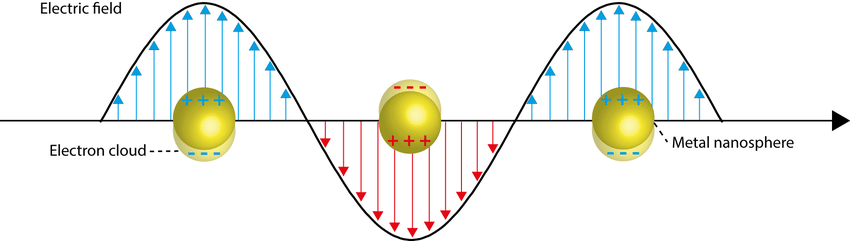
\includegraphics[width=\linewidth]{LSPR.png}
            \caption{Principle of interaction plazmon with electrical field, taken from \cite{20}}
            \label{fig:LSPR}
        \end{figure}

        This phenomena is used for plasmonic biosensors. There are two types of these biosensors, first one works on the principle of surface plasmon resonance and
        is made from thin film of noble metal. The second one uses the nanoparticles which are smaller than wavelength of light and their property of LSPR.
        Due to LSPR NPs are able to absorb and scatter light wiht high intensity. It is possible to observe it using dark-field microscopy. Thus these are highly
        applicable to biochemical sensors and cellular imaging. NPs are also useful as transducers because the scattering spectra depends on local refractive index
        and the spectra is shifted even with small changes of the refractive index. When the refractive index increases, the scaterring spectra shifts to red (bigger wavelength).
        It has also advantage in comparison with film biosensors because NPs can be used for very small volumes and gives better spatial resolution.
        The spectra of these NPs depends among other thinks on their size and shape. There are spherical NPs and nanorods which can be of various of aspect ratios (AR). \cite{1, 4, 33, 34}

        NRs are able to give two LPSRs (\ref{fig:GNR}) in comparison with spherical NPs, because the electrons can oscilate in two pathes. Oscillation of electrons inside the longer pathes
        (in longitudal dimension of the NR) is called longitudal resonance and produces light of longer wavelength, the other is called transversal resonance and
        produces light of shorter wavelength. GNR solutions can have various colors depending on their size and aspect ratio (\ref{fig:color}). \cite{4, 5, 6, 7, 8}
        For both NPs and NRs it is very important to know their sizes and shapes.
        
        \begin{figure}[h]
            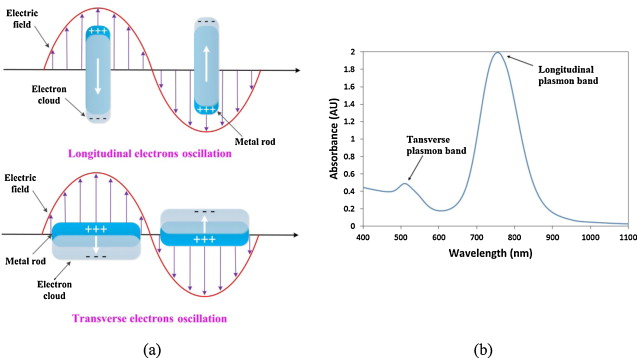
\includegraphics[width=\linewidth]{GNR.jpg}
            \caption{Principle of LPSR in GNRs, taken from~\cite{19}}
            \label{fig:GNR}
        \end{figure}

        \begin{figure}[h]
            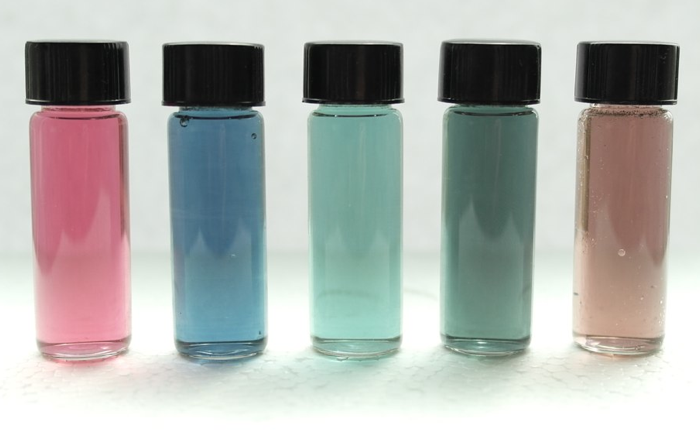
\includegraphics[width=\linewidth]{color.png}
            \caption{GNR solutions of different colors, taken from~\cite{32}}~\label{fig:color}
        \end{figure}

        One of the most common methods for determination of size and shape of AuNPs and GNRs~\ref{fig:GNR_shape} is transmission electron microscopy (TEM) which is very accurate and well-known technique.
        It is just necessary to make the images of the sample and using computer count the number and size of the NPs. But there are some disadvantages. For example,
        there is the complicated and nontrivial preparation of the sample, and the measurement itself can take a long time, as well as the requirement of the actual microscope itself.
        On the other hand, it can be used for every size and shape of AuNPs and even GNRs.~\cite{42}

        \begin{figure}[h]
            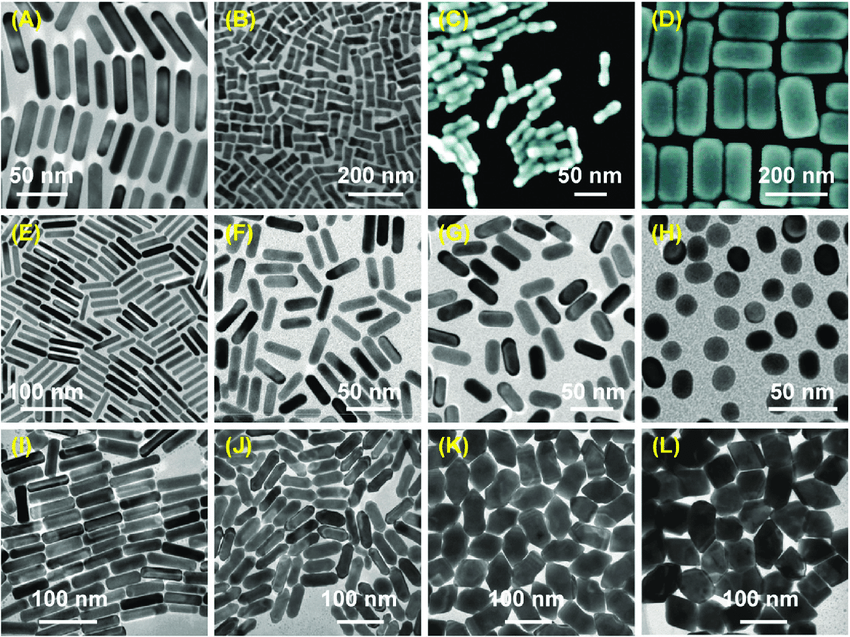
\includegraphics[width=\linewidth]{GNRs_shapes.png}
            \caption{TEM images of various shape and size GNRs, taken from~\cite{20}}~\label{fig:GNR_shape}
        \end{figure}

        The TEM microscope \ref{fig:TEM} works on the principle of electrons passing through the conductive sample and measuring the intensity of the beam that passes through.
        It consists of electron gun, system of lenses and fluorescent screen or digital detector.~\cite{7}

        \begin{figure}[h]
            \centerline{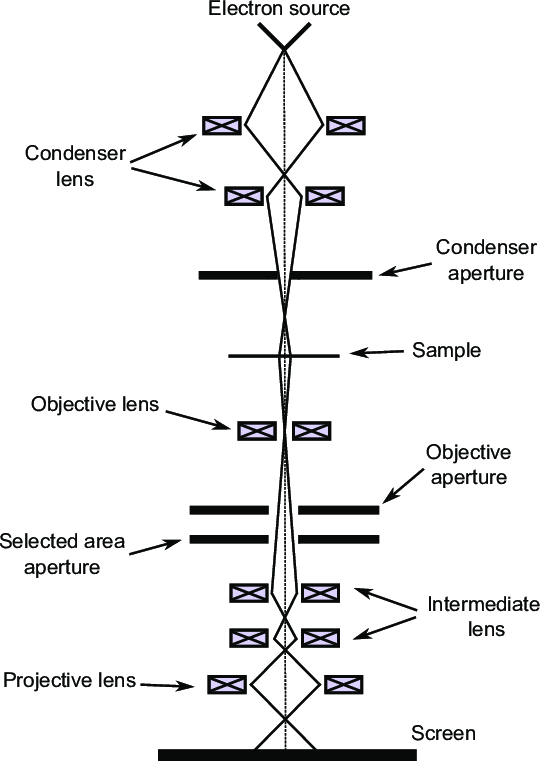
\includegraphics[width=250pt]{tem_principle.png}}
            \caption{TEM instrument schematic, taken from~\cite{20}}
            \label{fig:TEM}
        \end{figure}

        The electron gun is made of cathode which is heated and has negative potential. The potential is equal to the accelerating voltage. Then the is anode with positive potential.
        The electrons come from the cathode to the anode and passes through an axial hole in the anode. Then there are condenser lenses which are used for focusing the electron beam.
        In the most cases there are two lenses. First lens reduces image and the second focuses it onto the specimen. The specimen is made by measured sample and TEM grid.
        It is situated in specimen stage which can be taken out the microscope. Then there is objective lens which produces real image and projects it onto projector lens
        which produces enlarged image. There are more than one projector lenses due to the fact that one lens can provide just magnification 5:1
        and every next lens increases the magnification range. The last step is detecting the image. There are two options. The electron beam may be absorbed on the fluorescent screen
        which produces visible light. Or it may be detected by camera and displayed on the monitor and saved as .jpg image. \cite{7}

        With TEM it is more complicated, because the result can be obtained only after image processing. It is necessary to use segmantation methods to get number, sizes and shapes of
        NPs and NRs. Segmantation is image processing technique, which transforms image into regions, each representing one object, and includes deviding objects and background.
        Image processing can be divided into three layers, segmantation belongs to low layer, then there is image analysis which belongs to middle layer and image undestanding in high layer.
        There are plenty of methods of image segmantation but it is not easy to use them. Imgage segmantation is widely used in many diagnostic systems.
        It is used for automatic evaluation and quantitative analysis of microscopic and medical images. It is crucial that the segmantation is precise, becuase if it is not,
        the algorithm will not work. Segmantation lies in finding boundaries of objects, it can be cells, anatomical structures or nanoparticles.
        But there are more steps than the segmantation, the result has to be evaluated using another algorithms. There are more types of techniques, some of them are based on
        edge detection using discontinuities in pixel values. Another techniques find similarities in regions, there are technique like region growing, clustering and thresholding.
        There are, clustering methods, connectivity-preserving techniques and region-based methods which collects regions with similar intensity, color and texture, etc. \cite{1, 2, 15, 17}

        The most basic and even fast methods are region-based methods. This group includes for example threshold segmantation and regional grown segmantation.
        First mentioned technique is very simple and fast, it just divides pixels depending on threir value. thresholding does not take in account posision of pixel,
        it works just with its intensity. There are two types of thresholds, global threshold method has same threshold value for whole image and adaptive or local
        threshold method calculates the value for each point using average region intensity. Advantige of adaptive threshold is that it accommodates to inhomogenous
        lightning of image. There are various ways how to determine threshold value. thresholding can be also divided according to how many thresholds threre are.
        Bi-level thresholding is based on one threshold and divides pixels into two groups and multilevel thresholding selects multiple thresholds, thus there are several groups of pixels.
        One of the most used methods is called Otsu threshold~\ref{fig:otsu} and consist in finding value, where weighted within class variance is minimal. This method expects that histogram of image
        is bimodal, it means there is sufficient difference between background and region of interest intensity. \cite{15, 16, 17, 18}
        
        \begin{figure}[h]
            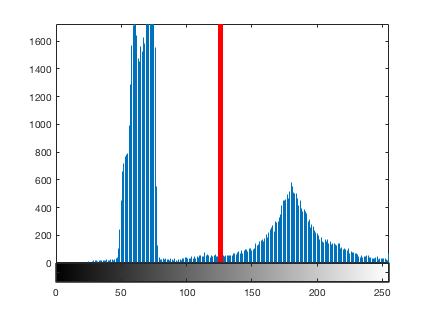
\includegraphics[width=\linewidth]{otsu_method.png}
            \caption{otsu threshold in bimodal histogram, taken from~\cite{20}}~\label{fig:otsu}
        \end{figure}

        There are also entropy-based techniques. Entropy is originally
        used in thermodynamics and it describes level of disorder of physical system. Shannon described entropy in informatics as unit for measuring efficiency of information in system.
        Entropic thresholding works on principle of finding threshold where sum of entropy of background and entropy of ROI is maximal. Another method is called minimum error thresholding
        and it considers histogram as probability density function which includes combination two populations, intensity of ROI pixels and of background pixels and
        it determines threshold as value, where overlap of these two population is minimal. It uses estimation of parameters of mean value, standard deviation and probability.
        This algorithm works with 2-D histogram, which can show relatiionship between two variables. There is also 2-D minimum error method which takes in account also position of pixel.
        multilevel thresholding determines more that one threshold and divides image into more levels depending on intensity and color (in RGB images). It is ideal for images with color
        inhomogenous background. Thus it is possible for example to assign both dark and bright pixels to zero and middle gray pixels to one. Disadvantage of these algorithms is
        it is often not possible to detect number of thresholds automatically. There are methods which can determine it using several times lowpass or highpass filters in image histogram
        to decrease or incease number of local maxina and minima.
        Another region-based type of image segmantation algorithms is called regional growth segmantation. It assumes that pixels of one region have similar values. Algorithm first selects
        seed pixel and then join similar pixels in neiborhood connected with this pixel into the region. It requires threshold value which is used as maximum difference between seed pixel
        and pixels assigned to the region. Disadvantage of these method is that it is slow and susceptible to noise.~\cite{15, 16, 17, 18}

        Another segmantation algorithm is called watershed segmantation algorithm (\ref{fig:watershed}) and is also region-based method. The name and even principle comes from nature and it is applied
        to grayscale or binary images. The goal of this algorithm is to find all connections in the image. connected pixels mean pixels that create one object (for example nanoparticle).
        First step of binary image works on principle of distance from nonzero pixel which creates distance map. Objects have to be of value zero and background of zero one,
        if it is reverse, image has to be negated first. In case of grayscale images the distance is calculated from local minima. So objects have to be of lower value than background.
        When distance map is calculated, watershed transform can be applied, it starts filling pixels from the highest value of distance and stops before two connected object join into one.
        It is called decomposition into catchment basins. Basins represente individual objects or regions. Every pixel of image is classified into one of the region or to background,
        so noise can be problem, because it creates large number of small regions. It is called over-segmantation. Thus image has to be filtered before applying watershed transform.~\cite{2, 3}
        
        \begin{figure}[h]
            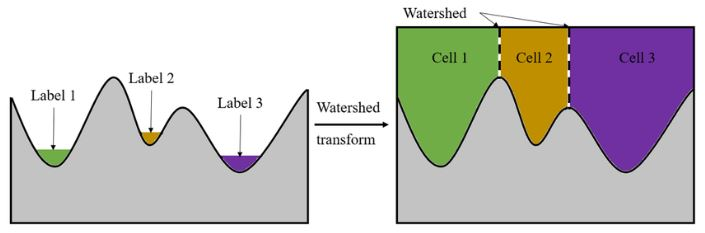
\includegraphics[width=\linewidth]{watershed.jpg}
            \caption{Watershed principle, taken from~\cite{20}}~\label{fig:watershed}
        \end{figure}

        Edge detection technique works on principle of finding local changes and discontinuities in the image~\cite{22}. It works with spatial domain instead of histogram in contrast with thresholding.
        Edge detection means detecting high frequencies in image, so it works like high-pass filter. Spatial frequency is generally number of cycles per distance, it has two components,
        frequency in x axis and y axis. In images it has units pairs of lines per milimeter, it means how quickly low value pixels shifts changes with high value pixels.
        This spectra can be obtained using discrete 2D Fourier transform, which is function of x and y. Thus high-pass filter extracts high frequencies and low-pass filter low frequencies \cite{23}.
        There are four types of edges, step edge where the value changes from one pixel to another, ramp edge, where the change is more gradual. Line edge have steep change
        but then returns to original value. Roof edge is made of slow change and in the peak value it also slowly returns back to original value.
        There are more steps in edge detection algorithm, filtering is used for removing noise. For example salt and pepper noise
        which means random white and black pixels in the image. It has to be very well balanced because filtering also reduces edge strange.
        Then there is enhancement phase which points up pixels with greater change of value. This step uses calculating gradient. Last step is called detection
        and it removes pixels with nonzero gradients which are nor edges.~\cite{3} Greater changes of value can be detected using differential operators which can calculate derivatives.
        There are several types of these descrete operators, Sobel and Laplacian operators are of the most used. Sobel operator calculates first derivative in each pixel.
        Tha algorithm uses two 3x3 matrices, transverse matrix which founds gradients in horizontal direction and longitudal matrix which founds gradients in vertical direction \cite{17, 22}.
        Then size of gradient is calculated using equation:

        \begin{equation}
            G = \sqrt{G_x^2 + G_y^2}
        \end{equation}~\cite{22}
        
        And vector of gradient can be calculated using equation:

        \begin{equation}
            \Theta = \arctan{\frac{G_x}{G_y}}
        \end{equation}~\cite{22}

        Zero angle corresponds with longitudinal edge, where pixels in left have lower value than ones in right.

        \begin{figure}[h]
            \centering
            \begin{bmatrix}
                -1 & 0 & 1\\
                -2 & 0 & 2\\
                -1 & 0 & 1
            \end{bmatrix}\hlinefill
            \begin{bmatrix}
                1 & 2 & 1\\
                0 & 0 & 0\\
                -1 & -2 & -1
            \end{bmatrix}
            \caption{Sobel operators, horizontal and vertical~\cite{22}}
        \end{figure}

        Another type of differential operator is called Laplacian operator and it is operator of second derivative and it detects zero-crossing of image intensity. It is more accurate
        than Sobel operator, but it detects isolated pixels better than edges, so it is not possible to use it to images with noise \cite{22}. Thus before using Laplacian operator it is
        necessary to perform low-pass filter, which reduces noise. For example median filter can be used, because it reduces noise while keep sharp edges.
        It is also possible to combine it with edge-matching filter, which has minimal response to isolated pixels and good response to merged edges \cite{21}. Due to this disadvantage,
        Laplacian operator is not frequently used. It consist from only one symetric matrix thus it is used for both directions. It can be also calculated using equation:

        \begin{equation}
            \nabla^2f = \frac{\partial^2f}{\partial x^2} + \frac{\partial^2f}{\partial y^2}
        \end{equation}
        \cite{22}

        \begin{figure}[h]
            \centering
            \begin{bmatrix}
                0 & 1 & 0\\
                1 & -4 & 1\\
                0 & 1 & 0
            \end{bmatrix}
            \caption{Laplacian operator \cite{22}}
        \end{figure}

        Clustering techniques work on principle of deviding pixels into various groups (clusters) depending on their characteristics. Cluster can be defined as group of pixels
        with similar properties with each other in same cluster and diverse with each other clusters \cite{26}. There are two types of clustering algorithms, hierarchical clustering
        is based on merging pixels with similar characteristics or spliting pixels with opposite characteristics and finds all possible combinations. Partitional clustering
        is iteration method with successive optimalization. hierarchical clustering can be divided into two groups, first is called agglomerative or bottom-up method and
        works on principle of merging data based on their similarities, first it defines every pixel as one cluster and then in every iteration merges similar clusters into one, until
        it reaches given number of clusters. Divisive or top-down method takes all pixels into one cluster and then in every cycle divides the most diverse pixels and from each clusters
        creates two \cite{25, 26} One of the most used clustering method is called k-means \ref{fig:k-means} and comes under partitional methods. Advantige of this method is that it is easy, fast and results are
        of high quality. Algorithm first randomly selects defined number (k) of cluster centers and assigns each pixel to the nearist cluster. In every iteration algorithm
        calculates for every cluster new center using mean value of all pixels in this cluster and then reallocates pixels depending on new distances from centers.
        Algorithm finishes when there is no significant change in centers \cite{26}. disadvantage of this method is that it is difficult to estimate k parameter.

        \begin{figure}[h]
            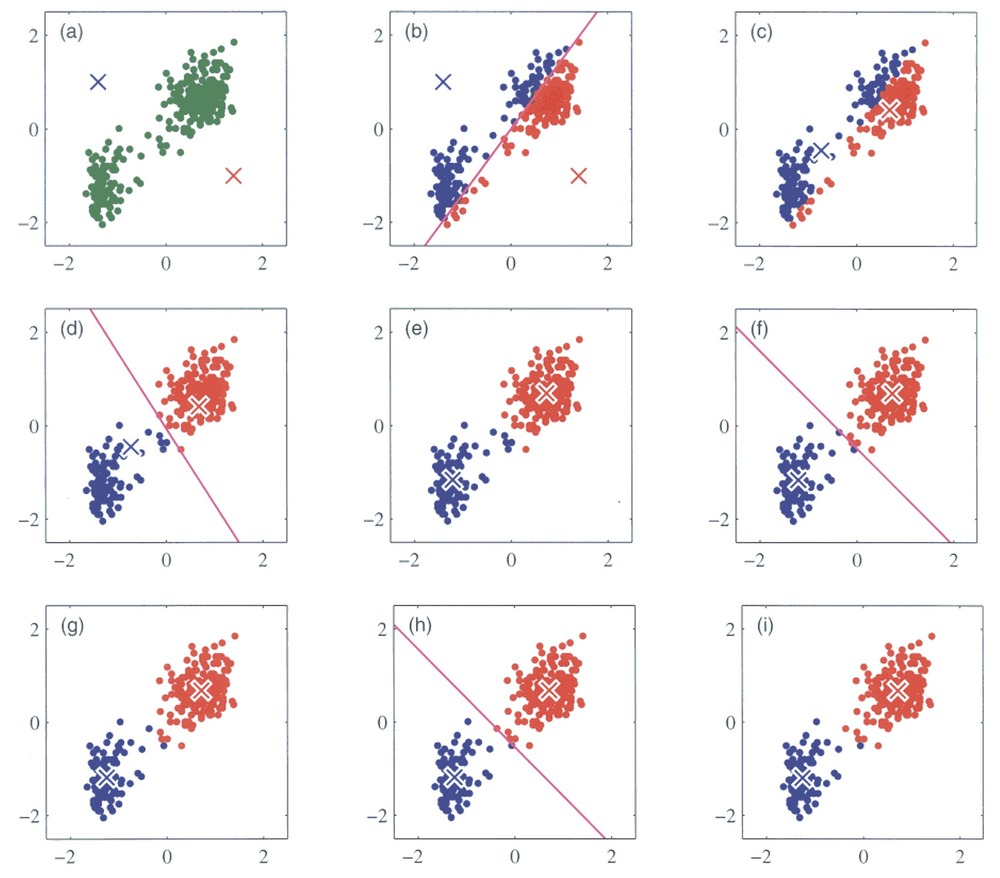
\includegraphics[width=\linewidth]{k-means.jpg}
            \caption{K-means principle, taken from \cite{24}}
            \label{fig:k-means}
        \end{figure}

        Another iterative algorithm is called fuzzy C-means clustering. It is based on fuzzy sets which does not assign each point just into one cluster, but instead of this,
        it calculates vector of memberships for each pixel, it means how strongly it belongs to each cluster. It has to be numbers between 0 and 1, sum of all memberships of one pixel must be 1.
        It is advantige in compare with k-means, because it allows overlapping of clusters. There si also defined number of clusters (c). Steps of C-means is similar as k-means,
        algorithm first randomly selects c centers, then calculates membership and updates cluster centers. Disadvantage is the same as in k-means,
        it is necessary to specify C parameter \cite{26, 27, 28}. There are more clustering algorithms, for example Gaussian clustering, but it has disadvantage, that is very complex.
        It is also iterative method and works on principle of calculating probability \cite{27}.

        There are also image segmantation techniques which use deep learning, wchich is subset of machine learning using neural network architecture with many layers.
        These systems requires large number of sample images and very good computating power. In biomedicine it is udes for example for automatic detectiion of cancer cells.
        Each neural network is composed from input layer, some amount of hidden layers and output layer. Deep learning neural networks may contain about 150 hidden layers
        in compared with traditional neural networks, wchich have 2-3. It can also learn automatically just from large datasets (2). Neural networks are formed from
        nodes which are connected with other nodes, these nodes are called neurons \ref{fig:neural_networks}. Each connection has weight, thus some of them are more important than others \cite{29}.
        Output of neuron can be calculated using equation:

        \begin{equation}
            y = f(\sum_{i=0}^{p} w_i x_i - \Theta)
        \end{equation}

        where \(y\) is output, \(x_i\) is i-th input, \(w_i\) is weigth of i-th input, \(f\) is activation function and \(\Theta\) is threshold of neuron \cite{29}.

        There are two types of operations, output of neuron can be linear function of weighted sum of inputs which in each connection multiplied by weight, the bigger is input,
        the bigger is output. Or there can be threshold and if weighted sum of inputs reaches this value, neuron becomes active and there is signal, which is multiplied in each
        connection with weight, otherway there is no signal. \cite{29}.

        \begin{figure}[h]
            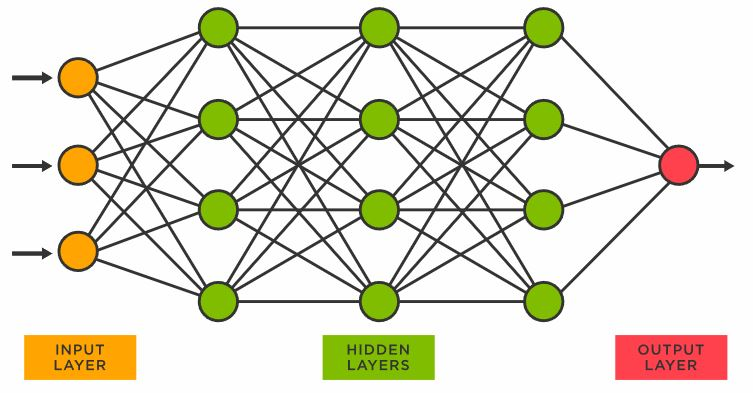
\includegraphics[width=\linewidth]{neural_network.jpg}
            \caption{Neural networks layers, taken from \cite{20}}
            \label{fig:neural_networks}
        \end{figure}

        Artificial neural network (ANN) is basic model of deep neural networks. It is composed of perceptrons, which means that signal moves just forward and output is connected to output.
        it uses back-propagation (feedback) to reduce errors while learning, during this it updates weights of connections. it is called adviser learning. \cite{30}
        Convolutional neural networks (CNN) are types of deep neural networks wchich are used for images, because it contains 2D layers. Ii learns directly from sample images \cite{2}.
        In CNN signal moves just forward thru all the hidden layers and output is connected with input thru these layers.
        CNN have three types of hidden layers, convolutional layer, which contains convolution of kernel matrix, which includes learned parameters, ant the image, it creates new matrix
        called activation map. This operation is applied by each layer in this group. pooling layer which merges each region into one value, there are more methods of this pooling function,
        it can be mean value, weighted value depending on distance from center pixel of region or max value of region, it reduces size of output thus computational complexity is decreased.
        Then there is fully connected layer, which connects all neurons from previous with each neuron from following layer. Then there usually are also nonlinear layers placed
        after convolutional layer,this layer uses non-linear operators to activation map. Prerequisite for this method is large number of relevant sample labeled images for training. \cite{30, 31}
        Recurrent neural network (RNN) are not feed-forward neural network, it means signal does not move just forward like in ANN and CNN. There is recurrent path which is able to affect input.
        it is connected with feedback, which figures like memory which connects sequence of data. RNN works previous data, so it can take it in account and output depends on it.
        These sequences of data represent in image processing spatial domain. \cite{30}

    \clearpage	
    \renewcommand{\refname}{Reference} 	% Přejmenování Reference
    (Nepodařilo se mi najít bibTex citace pro jiné zdroje než články, zatím jsem vložila jen ISBN pro knihy
    a odkazy pro webové stránky, do finální verze projektu to doplním.)
    \printbibliography
    \clearpage

\end{document}
        \clearpage
        
        \section{Goals}
        \pagestyle{plain}

The goal of the project is to create program for automatic determination of sizes and shape of nanoparticles and nanorods from TEM images. Particular goals are:

\begin{itemize}
  \item Prepare TEM samples with nanoparticles and nanorods.
  \item Get TEM images of nanoparticles and nanorods.
  \item Suggest proper segmentation method for TEM images.
  \item Create Python program for automatic analysis.
  \item Make GUI for the program.
\end{itemize}
        \clearpage
        
        \section{Methods}
        section{methods}

\pagestyle{plain}

subsection{Measurement}

subsection{Image analysis}

Another step is creating program in image analysis, it was writen in Python.
There were used several Python libraries, most of segmentation methods were
implemented using Scikit image library, there were also used opencv for Python
and Scipy ndimage for some functions, these libraries are using Numpy, which
is library used for work with martices. There was also used Matplotlib Pyplot
library for plotting and saving images.

First step after loading TEM image is convering it into grayscale due it could
be filtrated. TEM images can be of different scales and size and number of particles
in image depends on it. Median filter is used for denoising image. Filtrating works
of principle of convolution and size and appearance of convolution mask determine type
of filter. Median filter belongs to nonlinear filters which means that output is not
linear function of input. Median filter simply counts median value from neighborhood
of certain pixel for every pixel in image. Advantage of this filter is that it
preserv edges and removes noise. Size of kernel or pixel neighborhood depends on
scale of input image and also on type of particles because nanords are usually
smaller than nanoparticles so it has to be blured less.

Then grayscale image has to be transform into binary image. It is usually done
by finding appropriate threshold and pixels with value below threshold are 
transformed to zero and pixels with value above threshold are transformed into
one or 255 (it depends if binary image values are of type boolean with just 0 and 1
or 8-bit unsigned integer with values from 0 to 255). In case of this project
binary image is also inverted. In TEM images particles are black on white background
so in binary image particles pixels should be zero and background pixels should be one
and for this application it is better to invert it. There are several types of
thresholding techniques. Theese techniques uses histogram for calculating
appropriate threshold. There were used two different techniques in this project.
Minimum threshold method find pixel valu with minimum frequency in histogram and
this value is determined as threshold. Other method is called Otsu thresholding
and it is a bit more complicated algorithm. It consists in going throught every
pixel value and calculate variance in pixel values below this pixel and above this pixel
and finds pixel value with the smallest variance. This pixel value is determined as
threshold. Otsu thresholding is more advanced method and whould work better, but
in nanoparticles images with larger scale (there were just a few dart particles in center
of image) this method calculated too high threshold. More than just parctiles pixels
were determined as foreground. So it was chosen to use minimum thresholding method for
nanoparticles and Otsu thresholding method for nanorods.

After binarizing image there are used morphology operation to clean up image.
There are two basic operations called erosion and dilation. It works on principle
of interaction with structuring element which determines shape of pixel's neighborhood.
Dilation is used for filling holes and it increases size of objects. Algorithm changes pixel
value to one if there are enought white pixels in its neighborhood. Erosion is opposite
of dilation, it is used for removing small objects and it decreases size of objects.
Algorithm changes pixel value to zero if there are not enought white pixels in its
neighborhood. There are also two methods wchich consist of both erosion and dilation.
Opening first uses erosion and later dilation, it is used for removing small objects.
Closing first uses dilation and later erosion, it is used for removing small holes.
Opening and closing are better because it changes sizes of objects less than just erosion
and dilation. In scikit image library there are also fucntions designed perfectly
for removing small objects or holes. These scikit image function were also used
in this project for removing artifacts from background and fill holes in particles.

Main part of this project is image segmentation which separates particles so it could
be analyzed. There are plenty of methods used for segmentation and it is quite difficult
task to choose the best method and implement it. For this project watershed transformation
was chosen as main method. This algorithm starts with seeds and binary image. Seeds are
points or small clusters of points. In perferct world there should be one seed per
particle in image. Algorithm takes seeds and starts filling binary mask from theese points.
It is called watershed because seeds can be imagined as valleys (or local minima) and
algorithm fills every valley with water of different value starting from local minima.
It ends when it reaches edge of binary mask or when it meets water from another valley.
Labeled image is created, each pixel in one label has same number, background has zero.
There are more methods how to find seeds, in this project method called distance map
was used. It works on principle of finding for each zero pixel distance (number of pixels)
to the closest white pixel. Seeds were created by finding local maxima in distance fucntion.
It may happen that algorithm oversegments image so there are some small artifacts. So it
was decided to filter too small labels. It is done by algorithm calculates median of 
areas of labeles and going throught all labels and...

Watershed perfectly divides non-overlapping particles. In overlapping particles may occure
two cases, watershed divided particles well but did not count with their parts which
overlap, or it does not devide particles wll so it finds one big label. Due to this
problem it was decided to use also another segmentation method.
        \clearpage
        
        \section{Results}
        \pagestyle{plain}

\subsection{TEM images}\label{TEM_images}

TEM samples were prepared and TEM images were acquired. Various shapes and sizes of nanoparticles and nanorods were used. There were two samples of nanorods with unknown size and four sizes of nanoparticles with diameters 20 nm, 40 nm, 50 nm and 80 nm. There are examples of 20 nm nanoparticles (fig:\ref{fig:20nm}), 40 nm nanoparticles (fig:\ref{fig:40nm}) and nanorods (fig:\ref{fig:NRs}) with absorption peak on wavelength 800 nm.

\begin{figure}[h!]
\begin{center}
    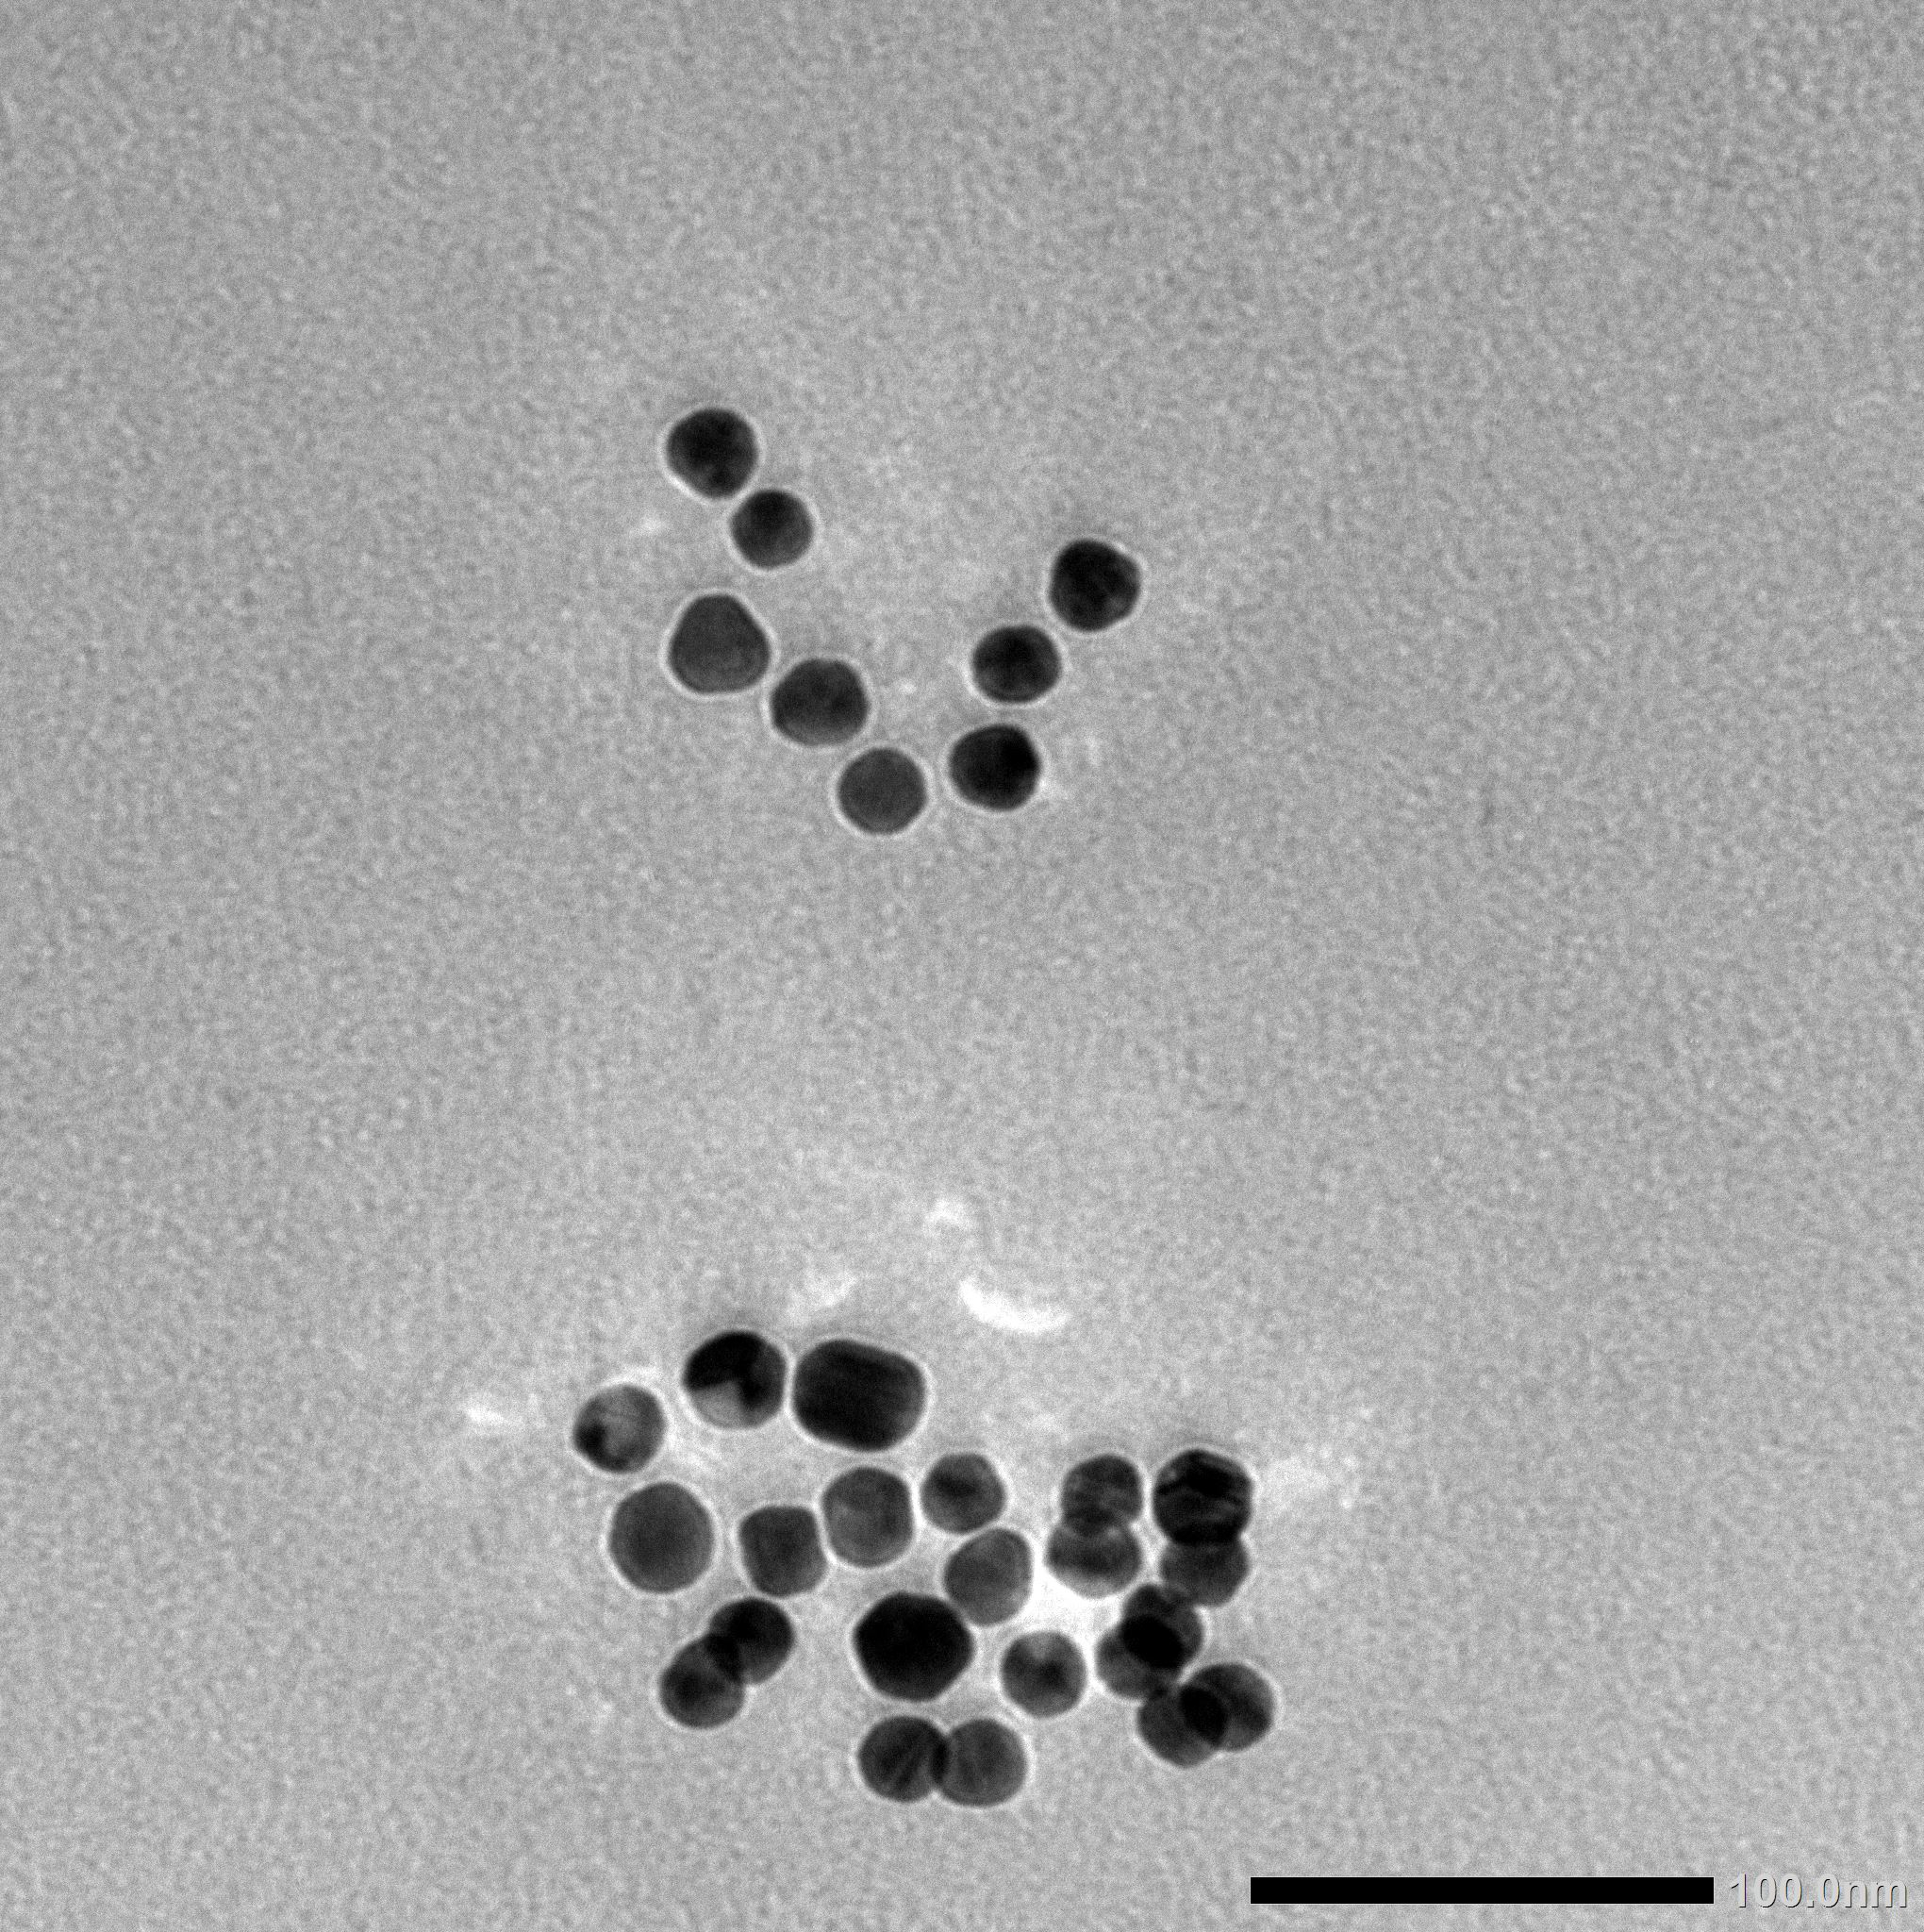
\includegraphics[width=0.5\linewidth]{20nm.jpg}
    \caption{Raw TEM image of 20 nm nanoparticles}~\label{fig:20nm}
\end{center}
\end{figure}

\begin{figure}[h!]
\begin{center}
\begin{subfigure}(a)
    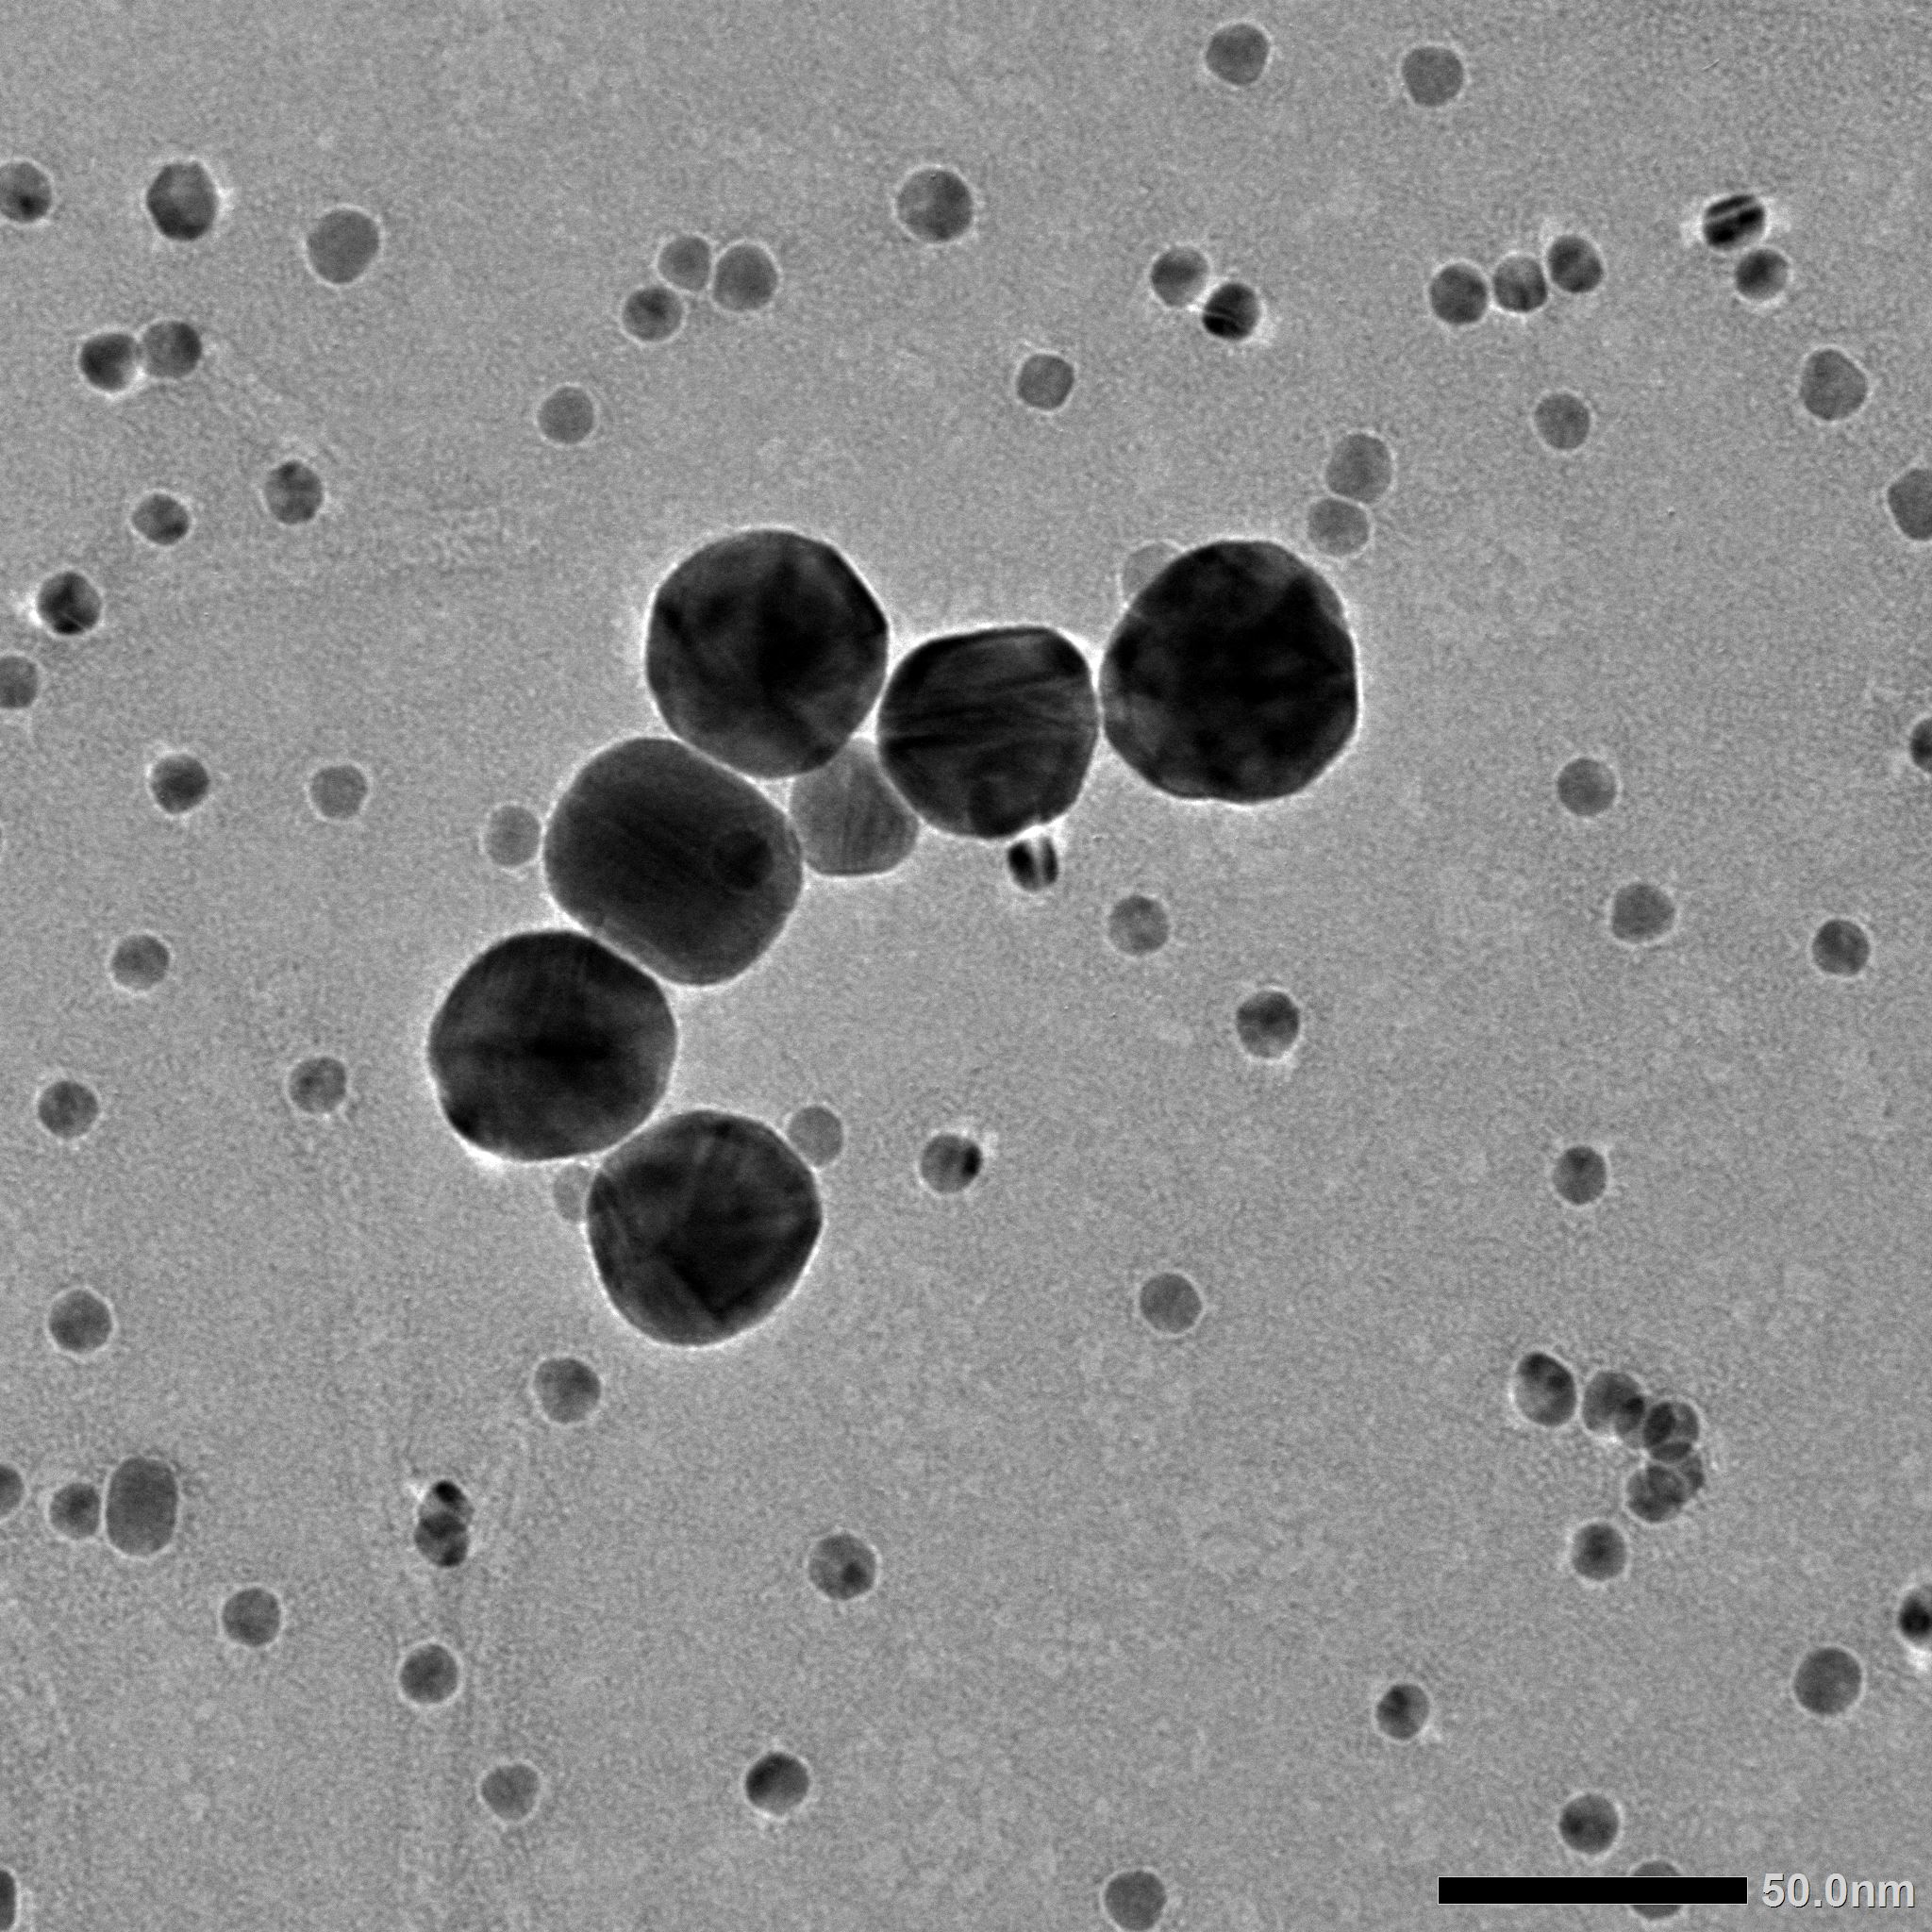
\includegraphics[width=0.4\linewidth]{40nm.jpg}
\end{subfigure}
\begin{subfigure}(b)
    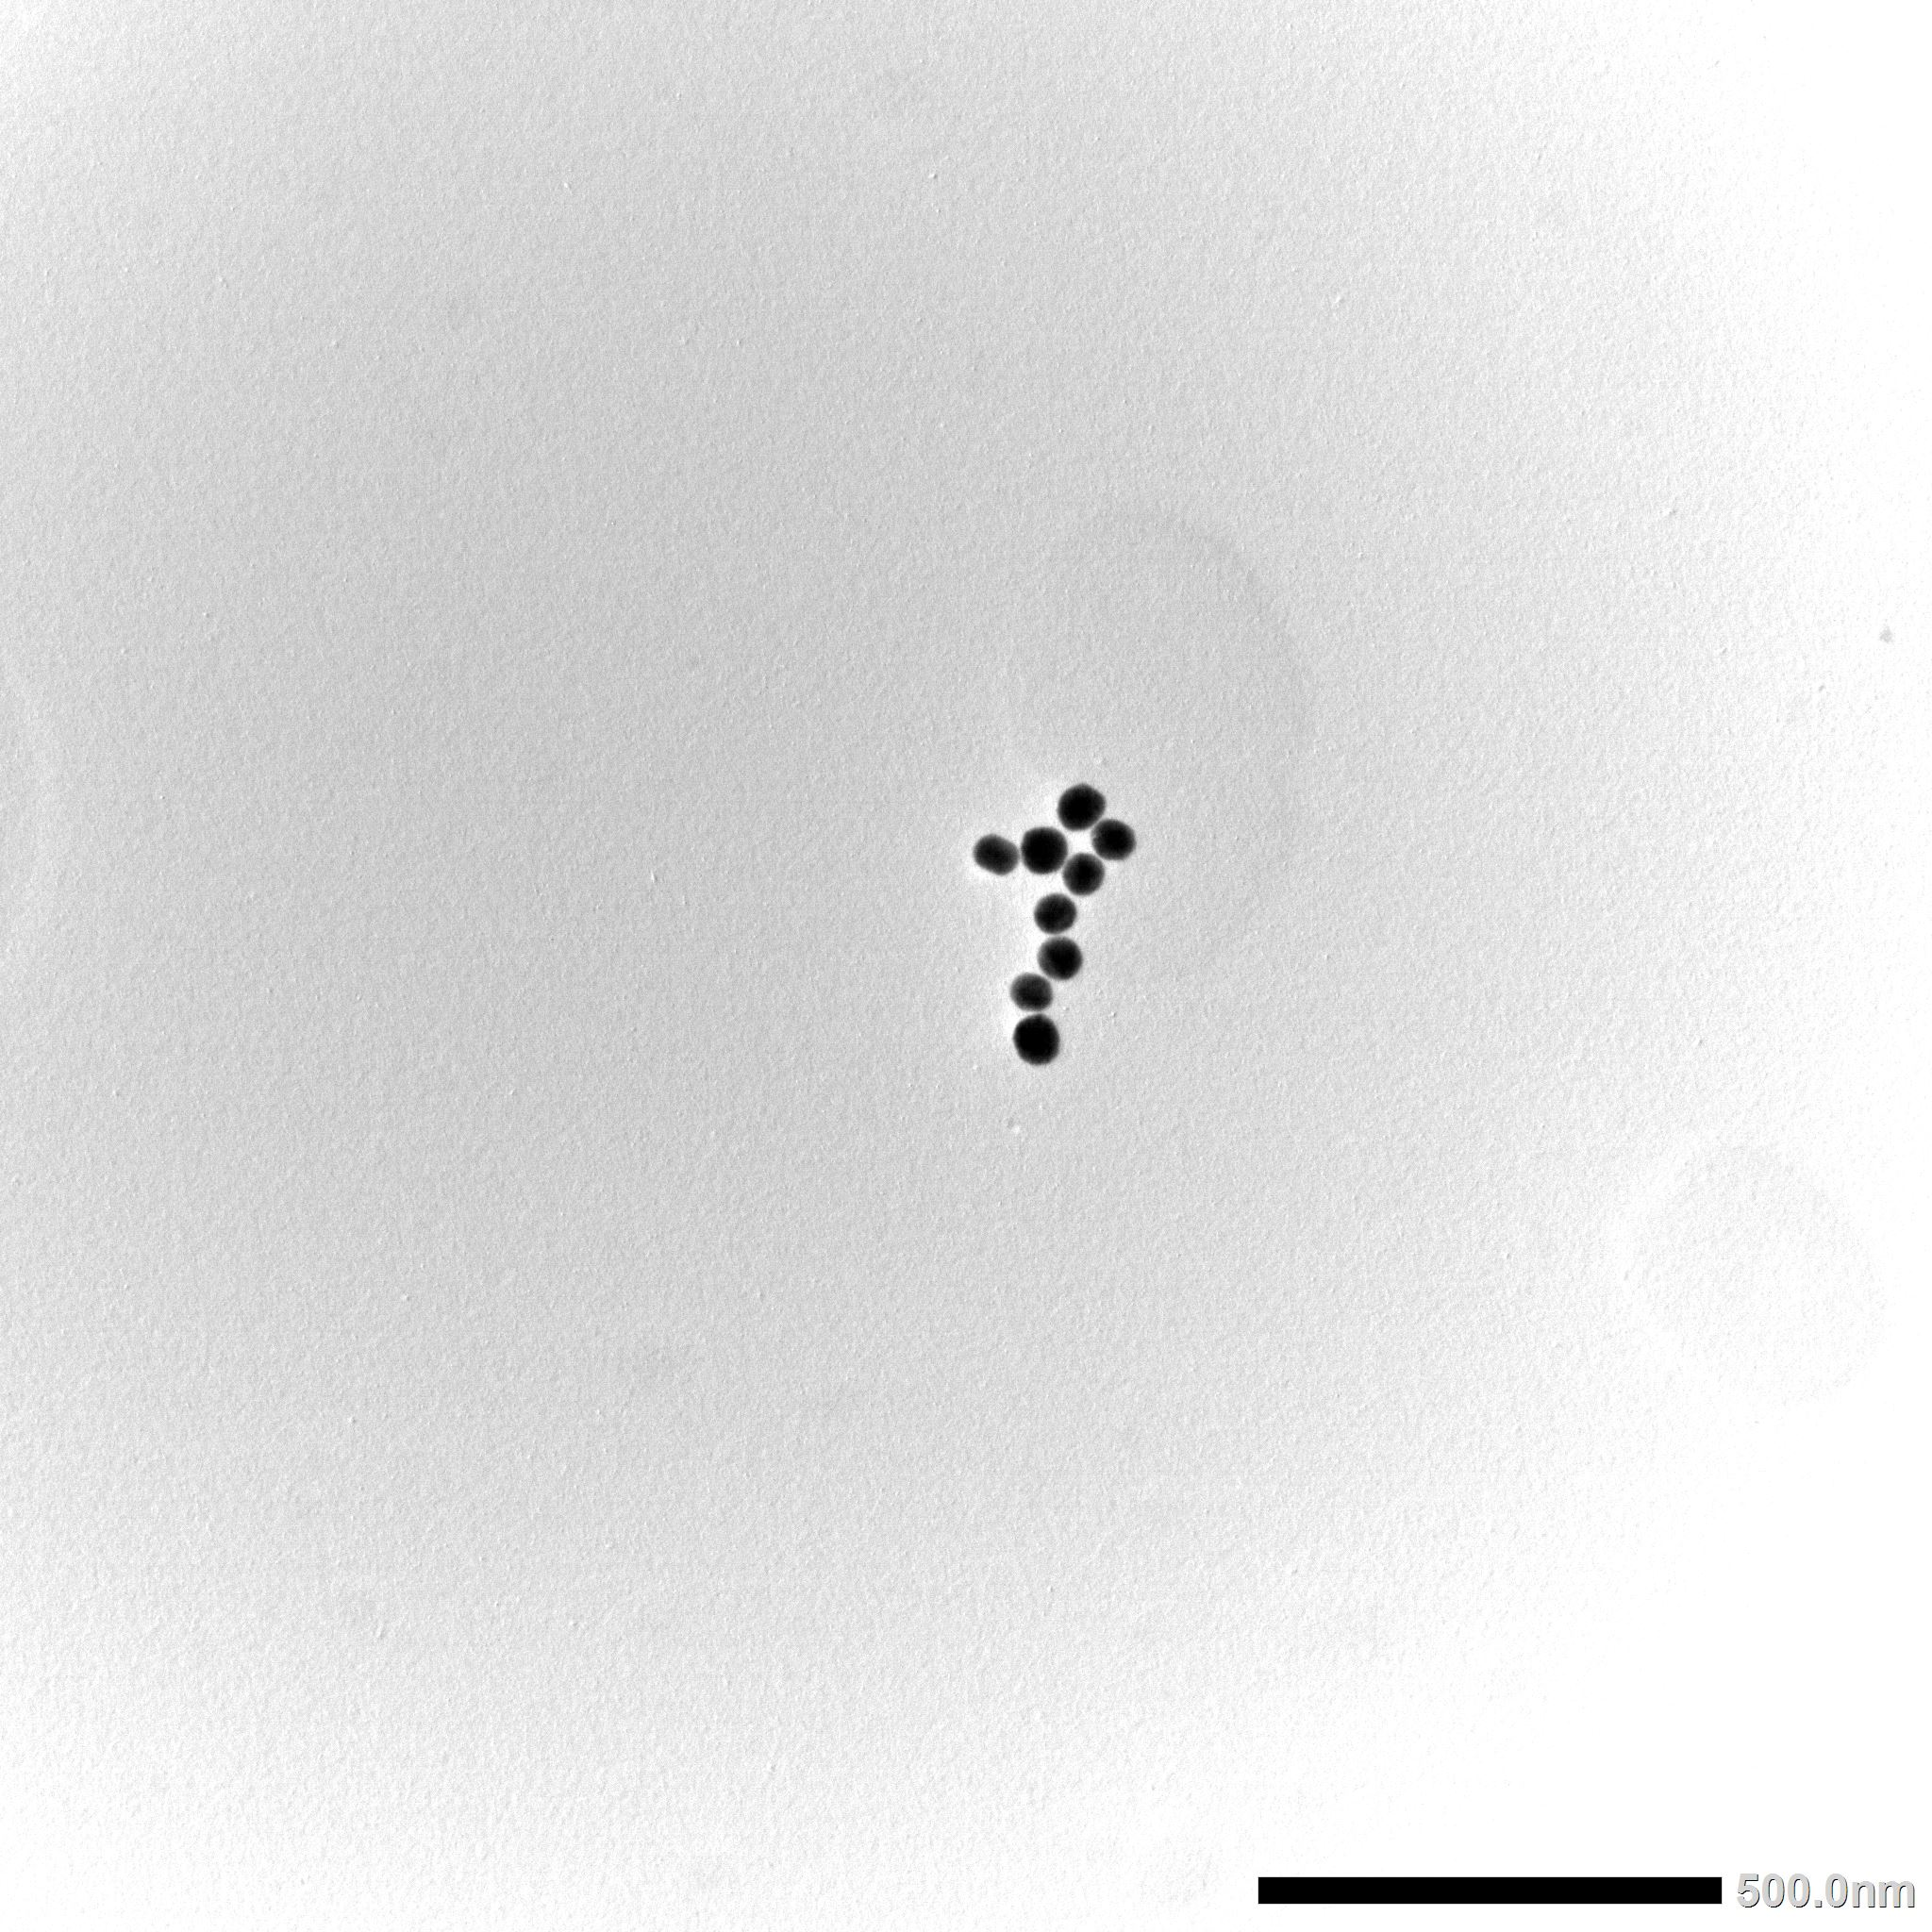
\includegraphics[width=0.4\linewidth]{50nm.jpg}
\end{subfigure}
\caption{Raw TEM images of 40 nm (a) and 50 nm (b) nanoparticles}~\label{fig:40nm}
\end{center}
\end{figure}

\begin{figure}[h!]
\begin{center}
\begin{subfigure}(a)
    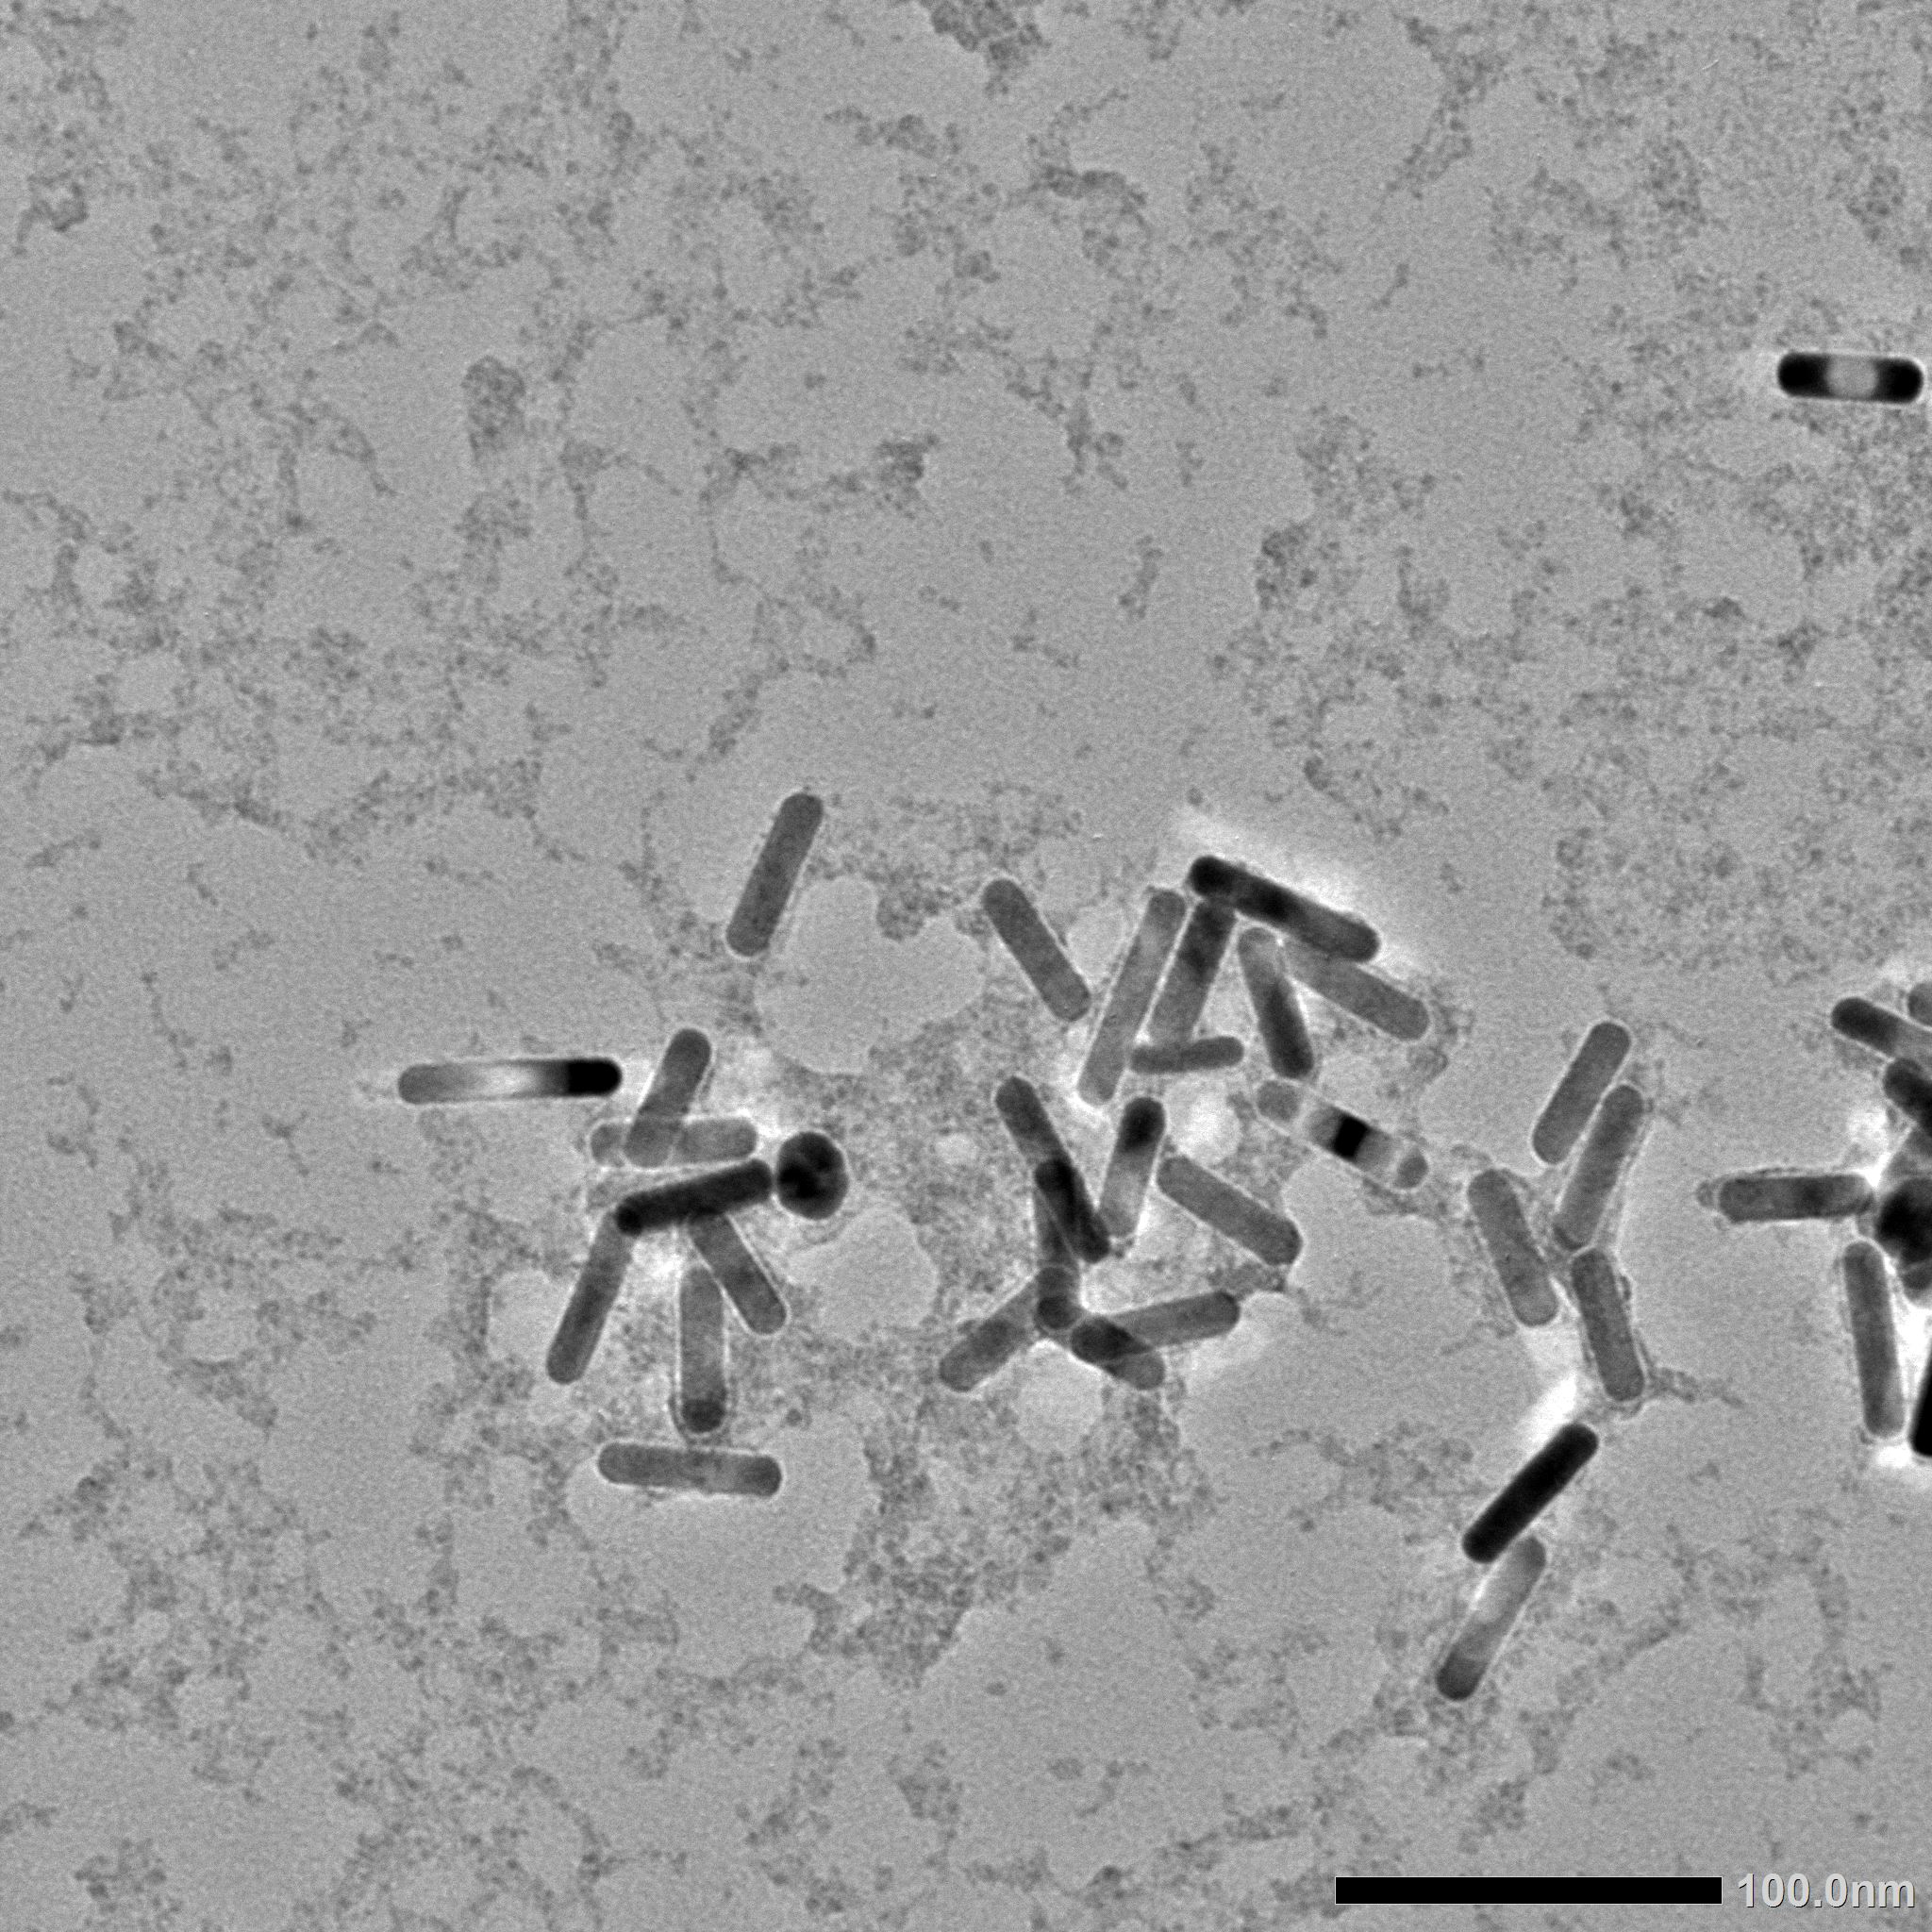
\includegraphics[width=0.4\linewidth]{NRs.jpg}
\end{subfigure}
\begin{subfigure}(b)
    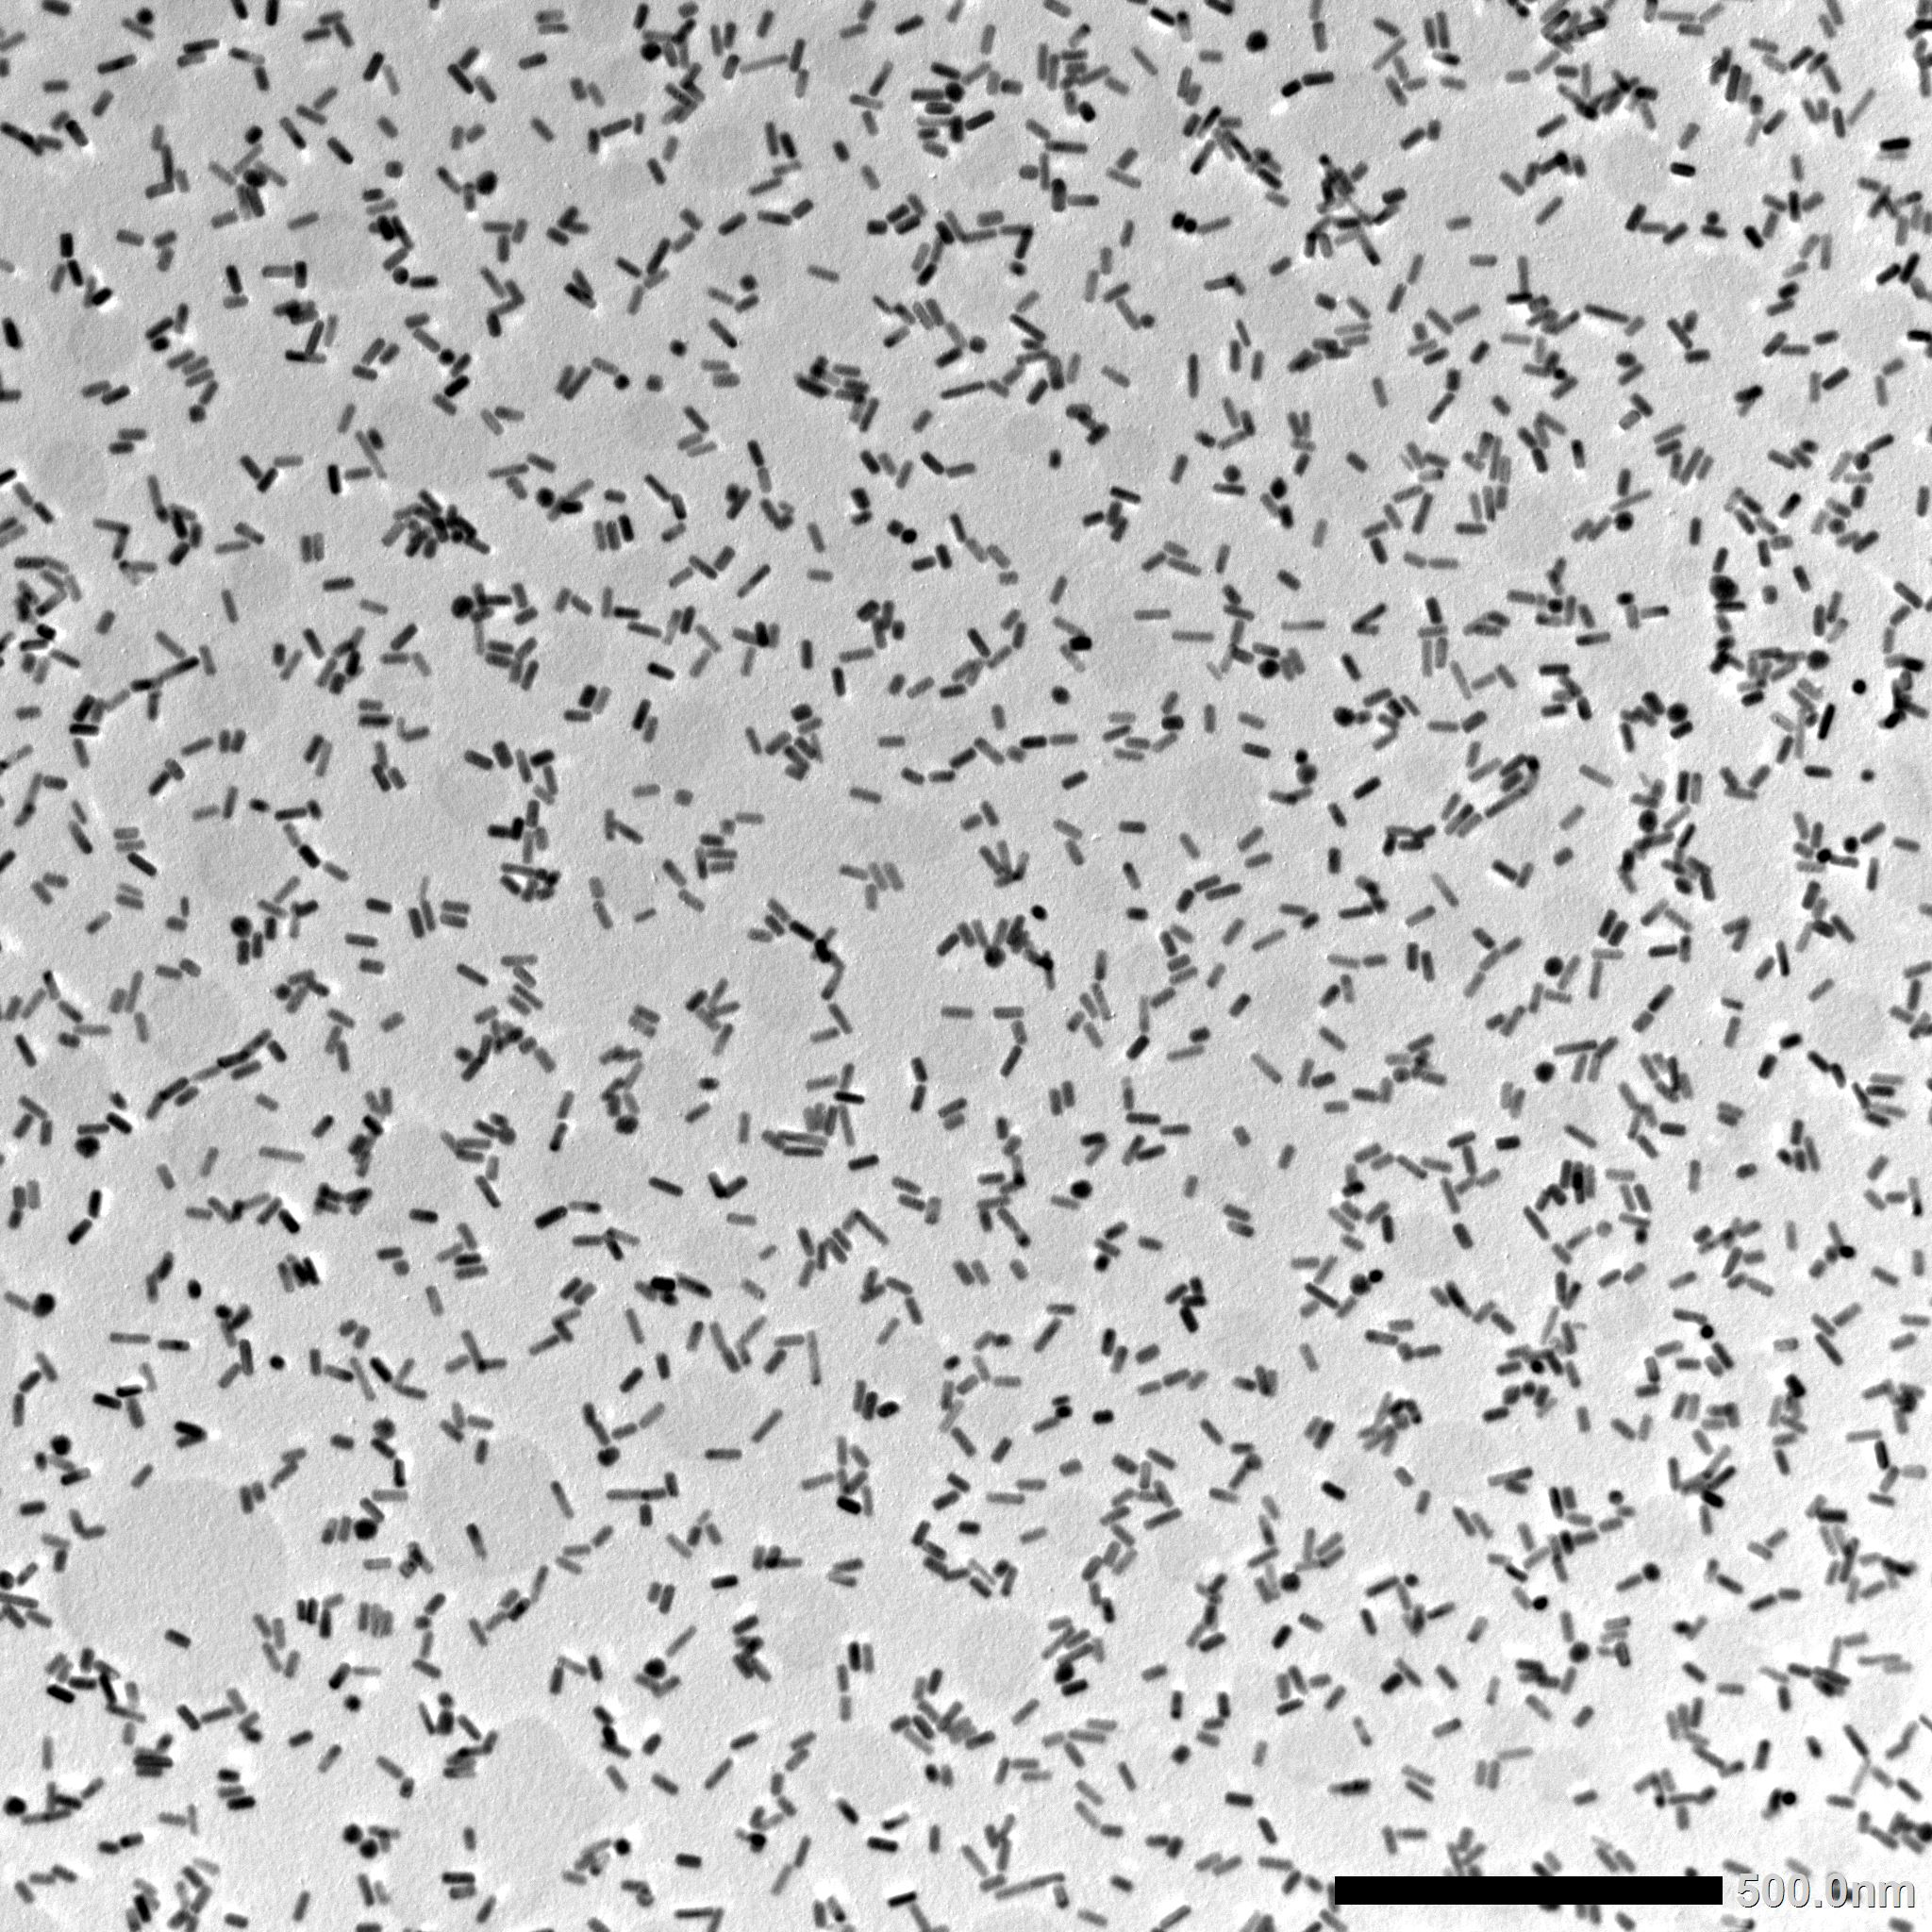
\includegraphics[width=0.4\linewidth]{NRs2.jpg}
\end{subfigure}
\caption{Raw TEM images of nanorods}~\label{fig:NRs}
\end{center}
\end{figure}

\subsection{Python program}\label{program}

Python program was created (see Attachement). Program is able to process more images at once and it can run from command line with arguments, user may define folder with images or decide if results should be plotted or not. Program requires metadata in json format, which includes information about type of particles (nanoparticles or nanorods) and scale of TEM image. Program perform image segmentation and returns labeled images, average sizes and histograms of sizes.

\subsection{Program outputs}\label{outputs}

Program was tested with various input data, examples of results can be seen on figures \ref{fig:res20nm}, \ref{fig:res40nm} and \ref{fig:resNRs}.

\begin{figure}[h!]
\begin{center}
    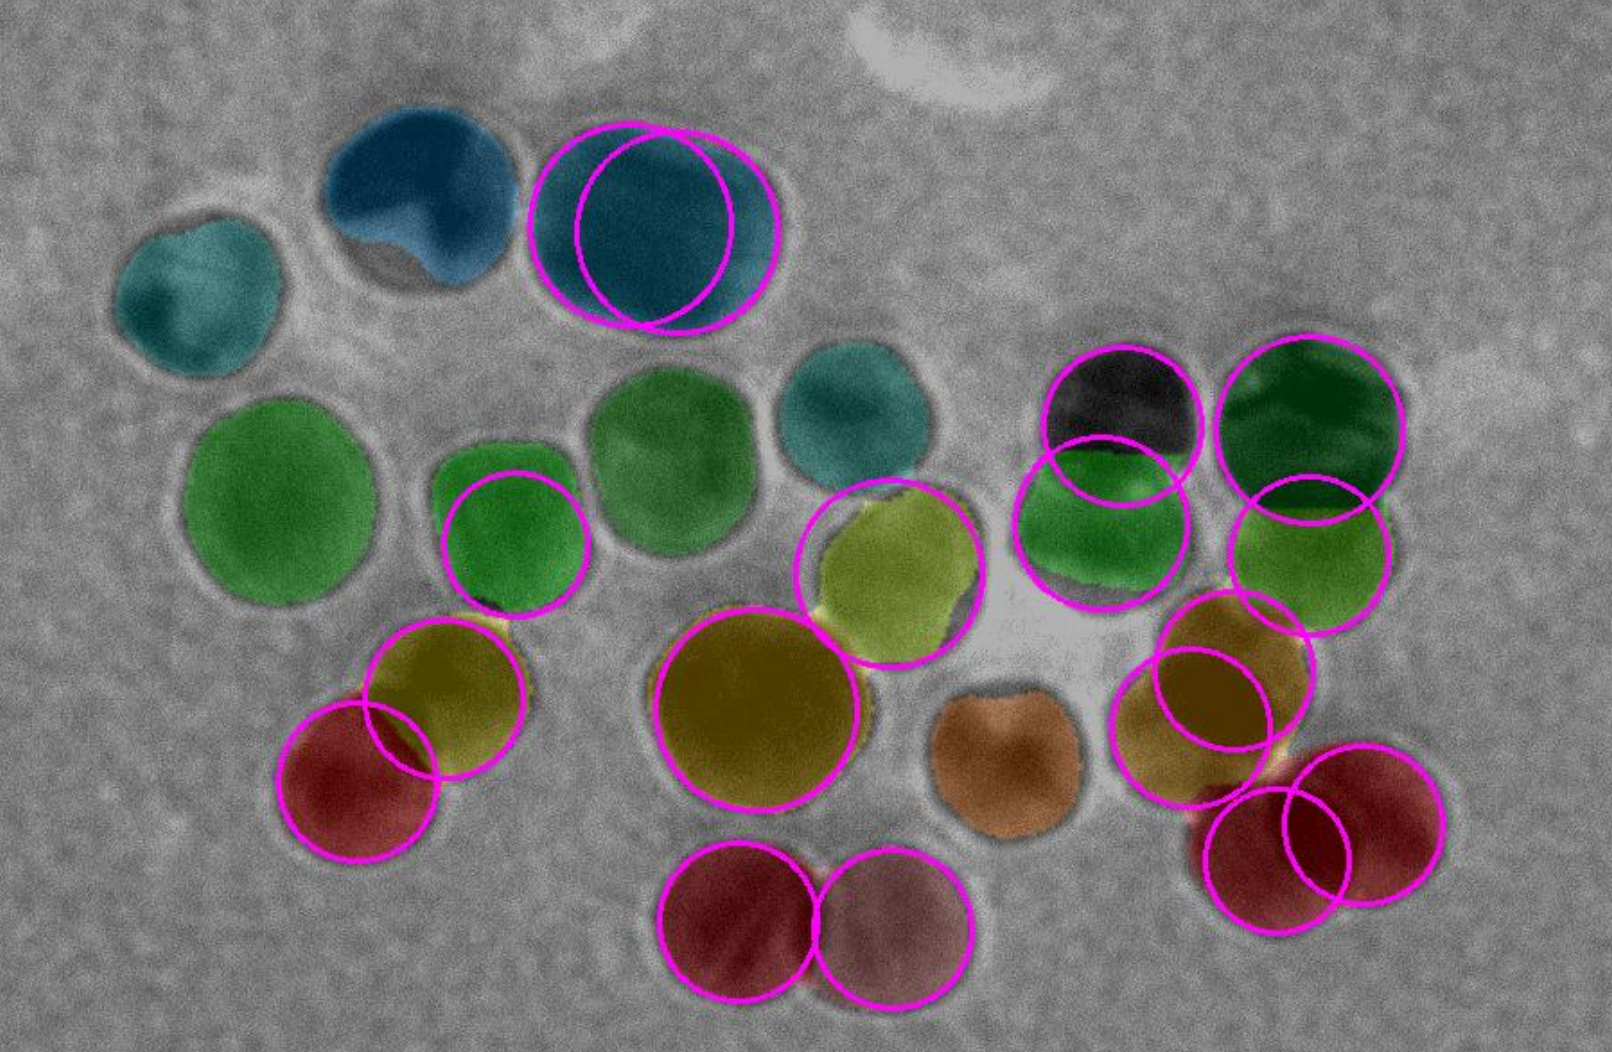
\includegraphics[width=0.5\linewidth]{res20nm.png}
    \caption{Croped result labeled image of 20 nm nanoparticles}~\label{fig:res20nm}
\end{center}
\end{figure}

\begin{figure}[h!]
\begin{center}
\begin{subfigure}(a)
    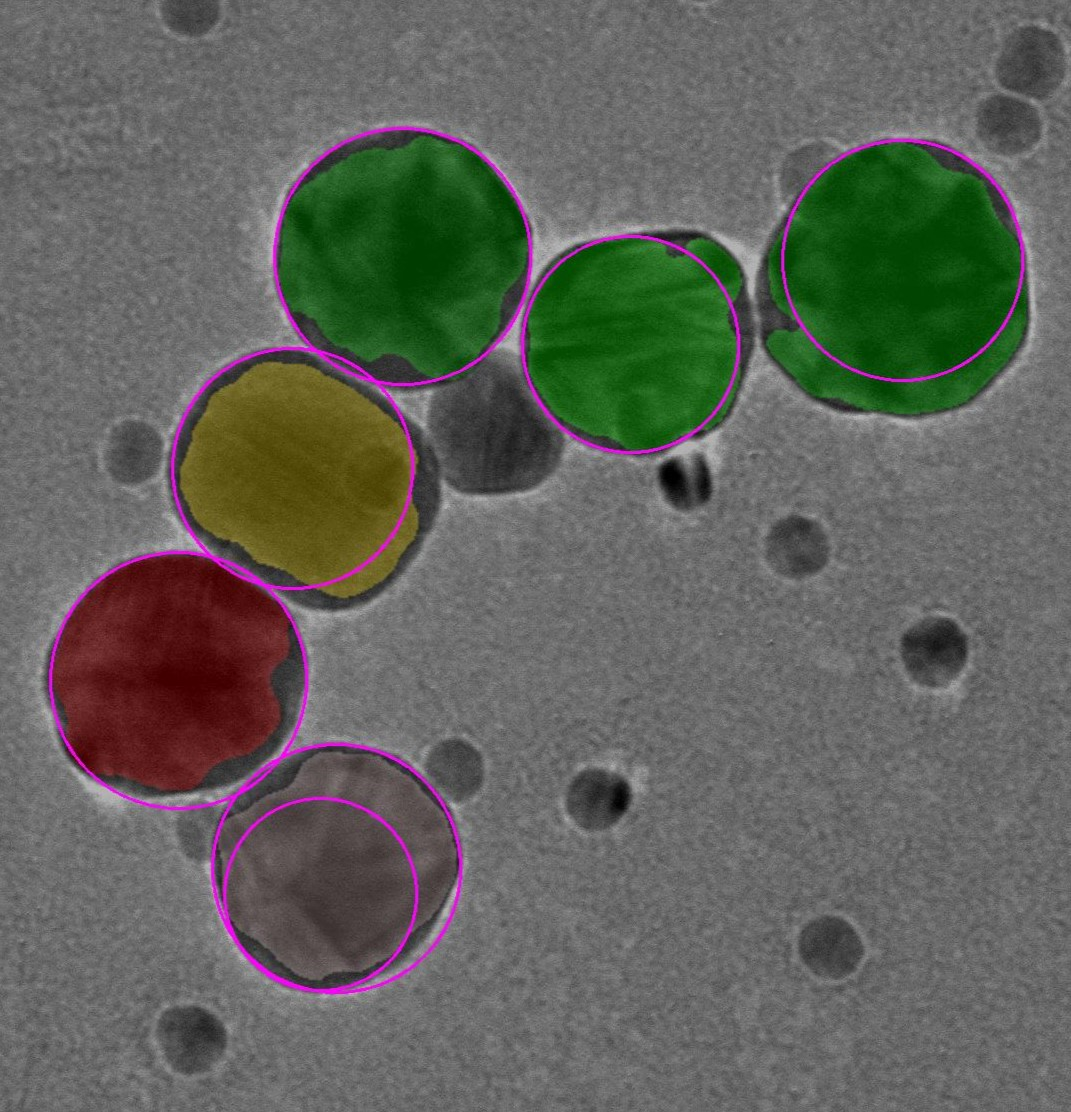
\includegraphics[height=200px]{res40nm.jpg}
\end{subfigure}
\begin{subfigure}(b)
    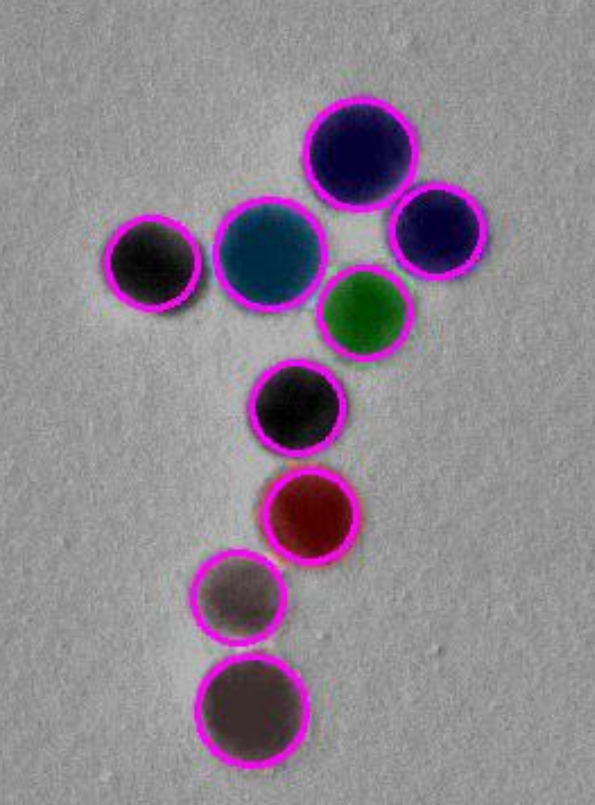
\includegraphics[height=200px]{res50nm.png}
\end{subfigure}
    \caption{Croped result labeled images 40 nm (a) and 50 nm nanoparticles (b)}~\label{fig:res40nm}
\end{center}
\end{figure}

\begin{figure}[h!]
\begin{center}
\begin{subfigure}(a)
    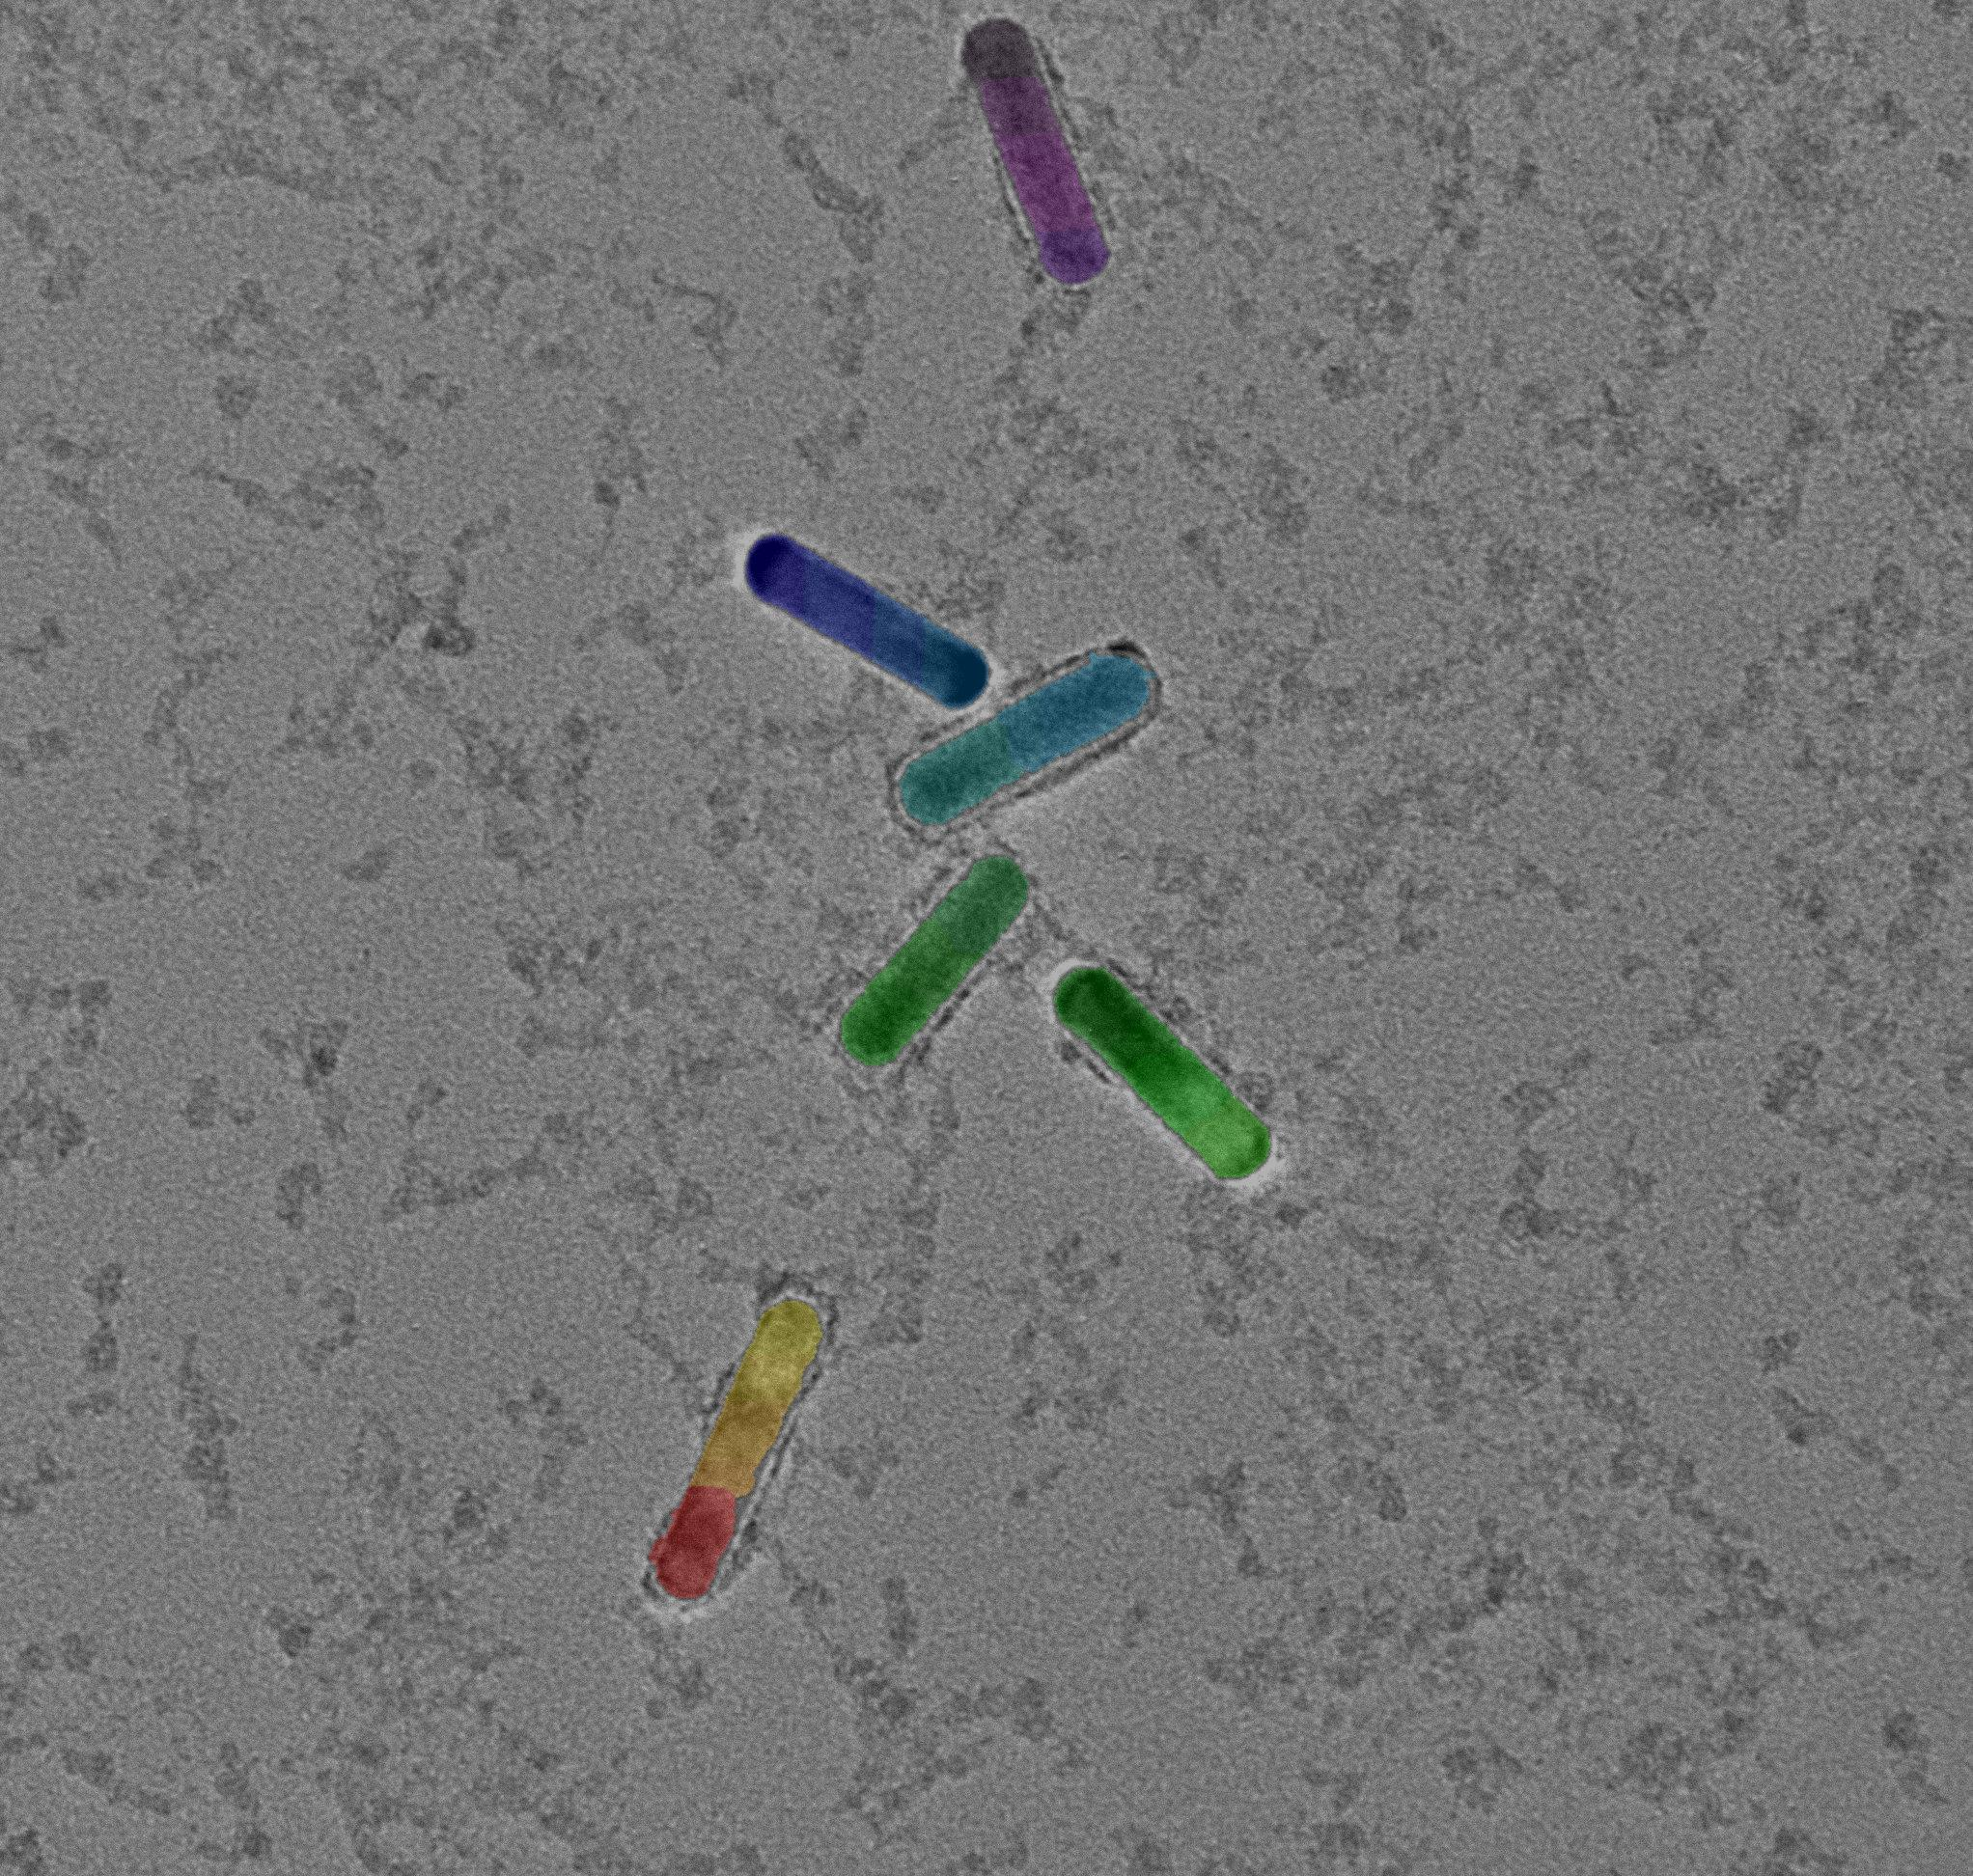
\includegraphics[width=0.4\linewidth]{resNRs.jpg}
\end{subfigure}
\begin{subfigure}(b)
    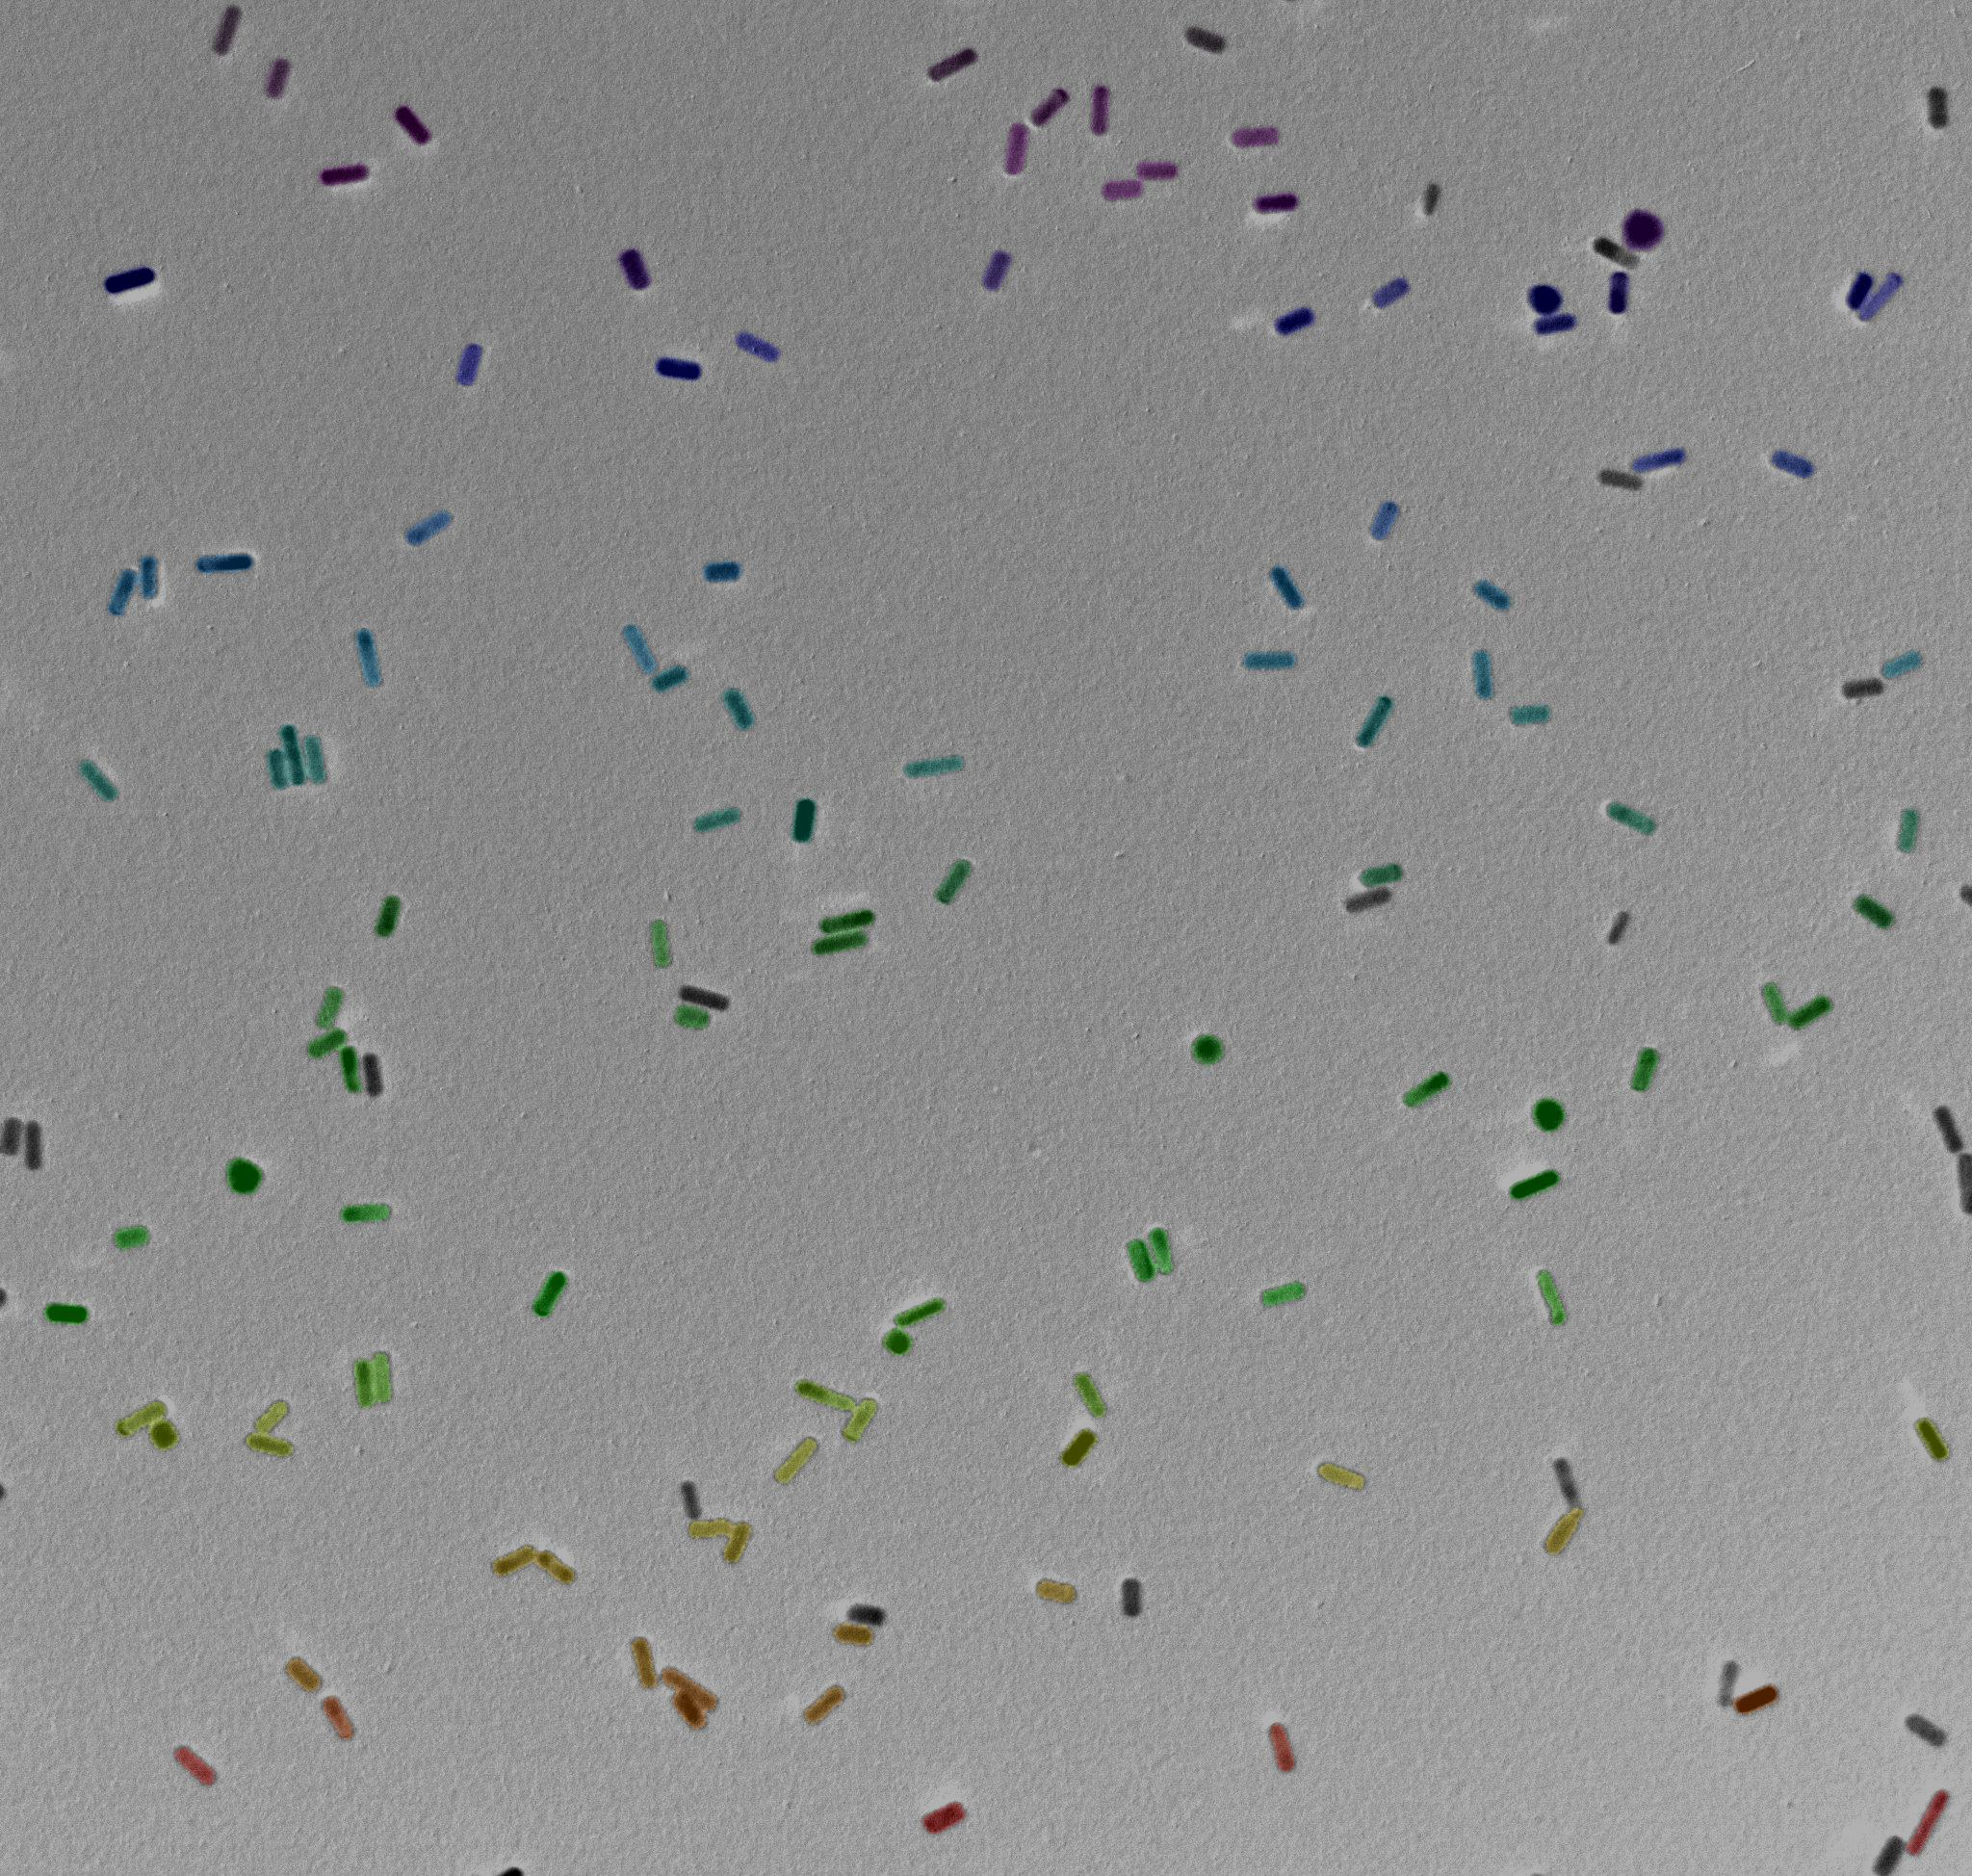
\includegraphics[width=0.4\linewidth]{resNRs2.jpg}
\end{subfigure}
    \caption{Result labeled image on nanorods with absorption peak on 800 nm (a) and 660 nm (b)}~\label{fig:resNRs}
\end{center}
\end{figure}

Histograms of sizes were calculated and plotted, histogram of nanoparticles shows layout of diameters in input image (fig:\ref{fig:hist20nm}) and histogram of nanorods shows major and minor axis lengths in input image (fig:\ref{fig:histNRs}).

\begin{figure}[h!]
\begin{center}
    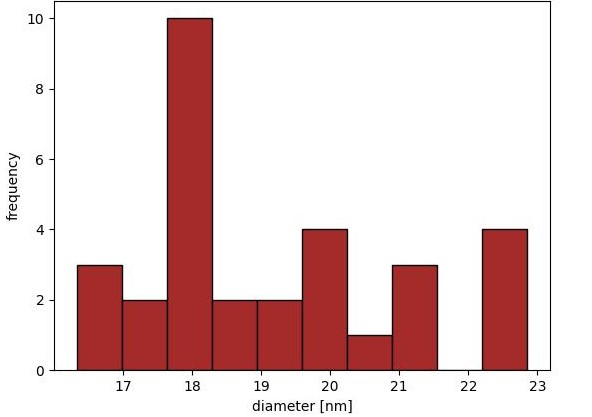
\includegraphics[width=0.8\linewidth]{hist20nm.jpg}
    \caption{Histogram of sizes of 20 nm nanoparticles}~\label{fig:hist20nm}
\end{center}
\end{figure}

\begin{figure}[h!]
\begin{center}
    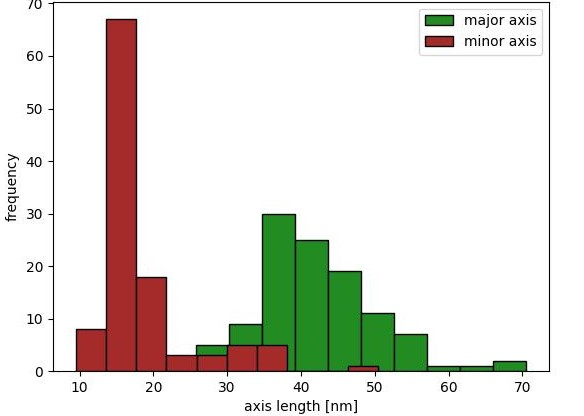
\includegraphics[width=0.8\linewidth]{histNRs.jpg}
    \caption{Histogram of sizes of nanorods with absorption peak on 660 nm}~\label{fig:histNRs}
\end{center}
\end{figure}
        \clearpage
        
        \section{Discussion}
        \pagestyle{plain}

\subsection{Results evaluation}

Main result of this project is Python code for automatical analysis of TEM images of gold nanoparticles and nanorods. This code was debugged using input image \ref{fig:20nm}, because it is the most ideal image, there are advantages of this image: pretty good resolution, number of particles, fairly good contrast and homogeneous background. This image has also imperfections which can be used for solve these frequent issues, which are overlapping particles, hight resolution of image and small bright spots on particles. Overlapping particles were solved by using combination of two segmentation methods. Watershed transform was used for find all particles, but watershed divides ovelapping particles in the middle so it decreases its area, in some cases it even cannot divide some particles. So hough transform which finds specific shapes in image is used for detecting circles, this method is used just for areas with ovelapping particles. High resolution issue and bright spots are descibed in chapter \ref{image_errors}. Result of this sample image can be seen on figure \ref{fig:res20nm} and histogram of sizes of this image can be seen on figure \ref{fig:hist20nm} in chapter Results.

\subsection{Sample preparation errors}\label{measurment_errors}

The goals of the project were to prepare TEM samples on copper gird and acquire TEM images. Samples of nanoparticles and nanorods were prepared, but during TEM measurment there were another small particles on some samples. Theese small particles were DNA fragments and it means that some of grids must be used before and returned into box with new grids. This accident may cause errors during image segmentation while theese small particles are not removed well. This false detection of DNA particles can be seen on figure \ref{fig:res50nm}.

\begin{figure}[h!]
\begin{center}
    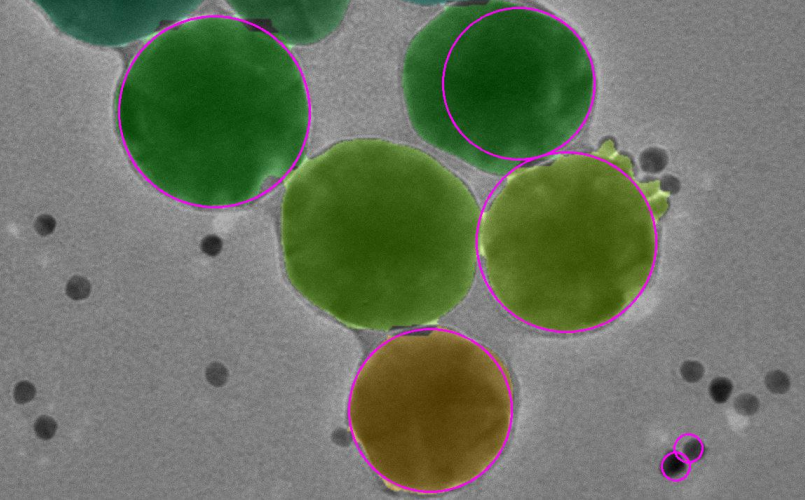
\includegraphics[width=0.5\linewidth]{res80nm.png}
    \caption{False detection of DNA particles in 80 nm nanoparticles TEM image}~\label{fig:res50nm}
\end{center}
\end{figure}

Another source of segmentation errors may be insufficiently dried samples. Samples of nanorods with absorption peak 800 nm can be seen on image \ref{fig:NRs}, this iimage has inhomogeneous background due to it was measured while sample was still a little wet. This is error which may happen more frequently so it is treated in software, however it declines quality of image. Wet sample can be seen on figure \ref{fig:wet}.

\begin{figure}[h!]
\begin{center}
    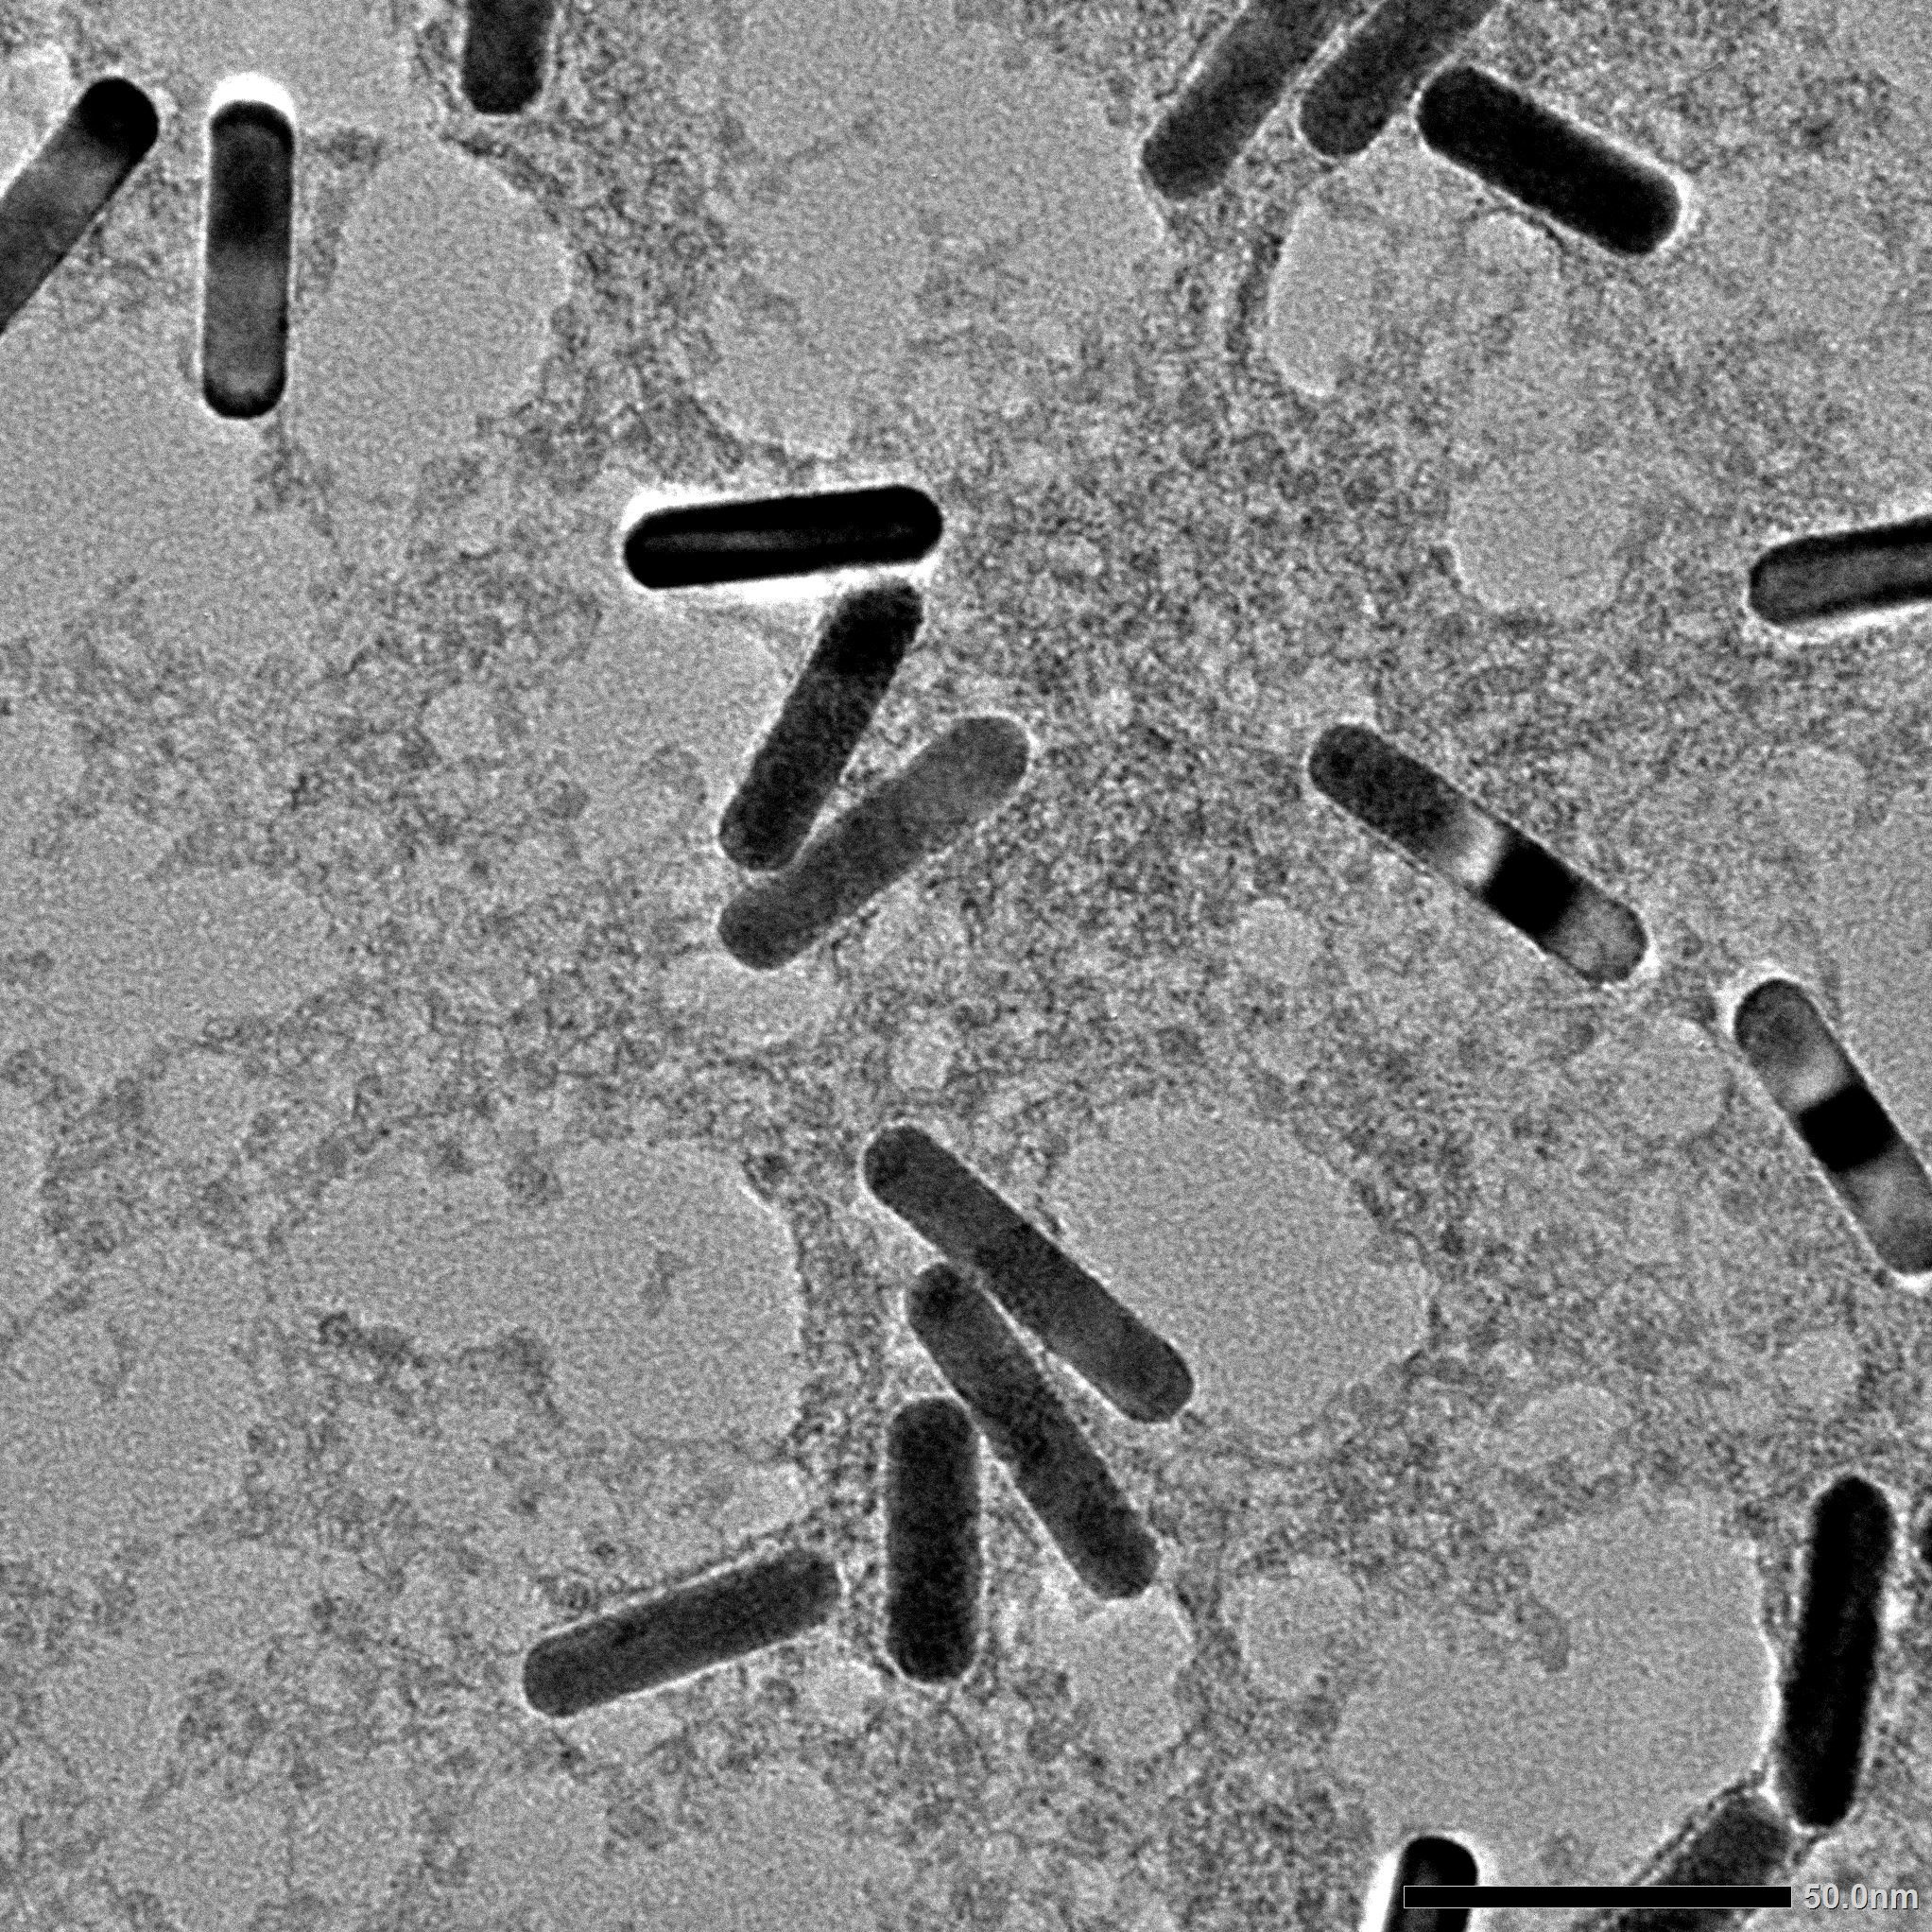
\includegraphics[width=0.5\linewidth]{wet.jpg}
    \caption{Inhomomogeneous background caused by wet sample}~\label{fig:wet}
\end{center}
\end{figure}

\subsection{TEM measurment errors}\label{image_errors}

Another sources of potential errors can by quality of TEM images. There are several issues which affects results of image analysis program. First issue is resolution. Microscope computer saves images in very high resolution 2044 x 2044 pixels and due to computational complexity of most functions, image resolution has to be reduced. For most of images rescaling does not matter, but there are images where particles are very tiny in compare with image size (example of this case can be seen on figure \ref{fig:40nm} (b) or figure \ref{fig:NRs} (b) in chapter Results). After rescaling theese particles have diameter for example 8 or 9 pixels, so accuracy of measurement extremely decrases. Solution for this problem could be manually cropping thees images before automatical analysis, but there is an issue. Images contain scale bar and it is located in corner of image and it is used to determine pixel size, so cropping image would remove this information. Appropriate solution for this problem was not found and it will be part of following project.

Another issue with TEM images quality can be contrast. Algorithm for particles analysis works on principle of substracting particles from background based on pixel intensity. Particles in some images contain stains with higher intensity which is similar or even higher than background intensity. So algorithm assigns these pixel to background not to particles. This issue is partly treated in code by using morfological operation for filling holes. This solution can solve smaller bright spots but it cannot do anything with cases where for example half of particle is bright. Some TEM images have low contrast overall so thresholding methods may not be so accurate it could be. Example of low contrast nanorods with even bright spots can be seen on \ref{fig:resNRs} (a) in chapter Results. In this image wet background is also problem, so it decreases quality of image even more. Bigger bright spots may cause oversegmentation of image. This case can be seen on figure \ref{fig:oversegment}.

\begin{figure}[h!]
\begin{center}
    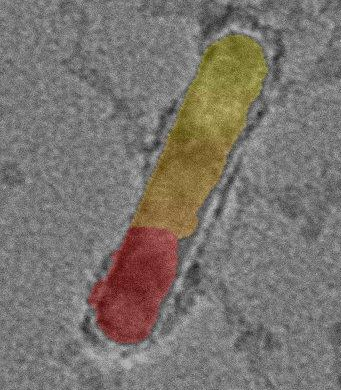
\includegraphics[width=0.5\linewidth]{oversegment.png}
    \caption{Oversegmented nanorod}~\label{fig:oversegment}
\end{center}
\end{figure}

Last issue which is related to image quality and occured in sample images is badly focused image. It is problem especially in images with large number of small particles, because particles in samples are overlapping and in this case it is almost impossible to divide them well. Example of this case can be seen on figure \ref{fig:bad_focus}.

\begin{figure}[h!]
\begin{center}
    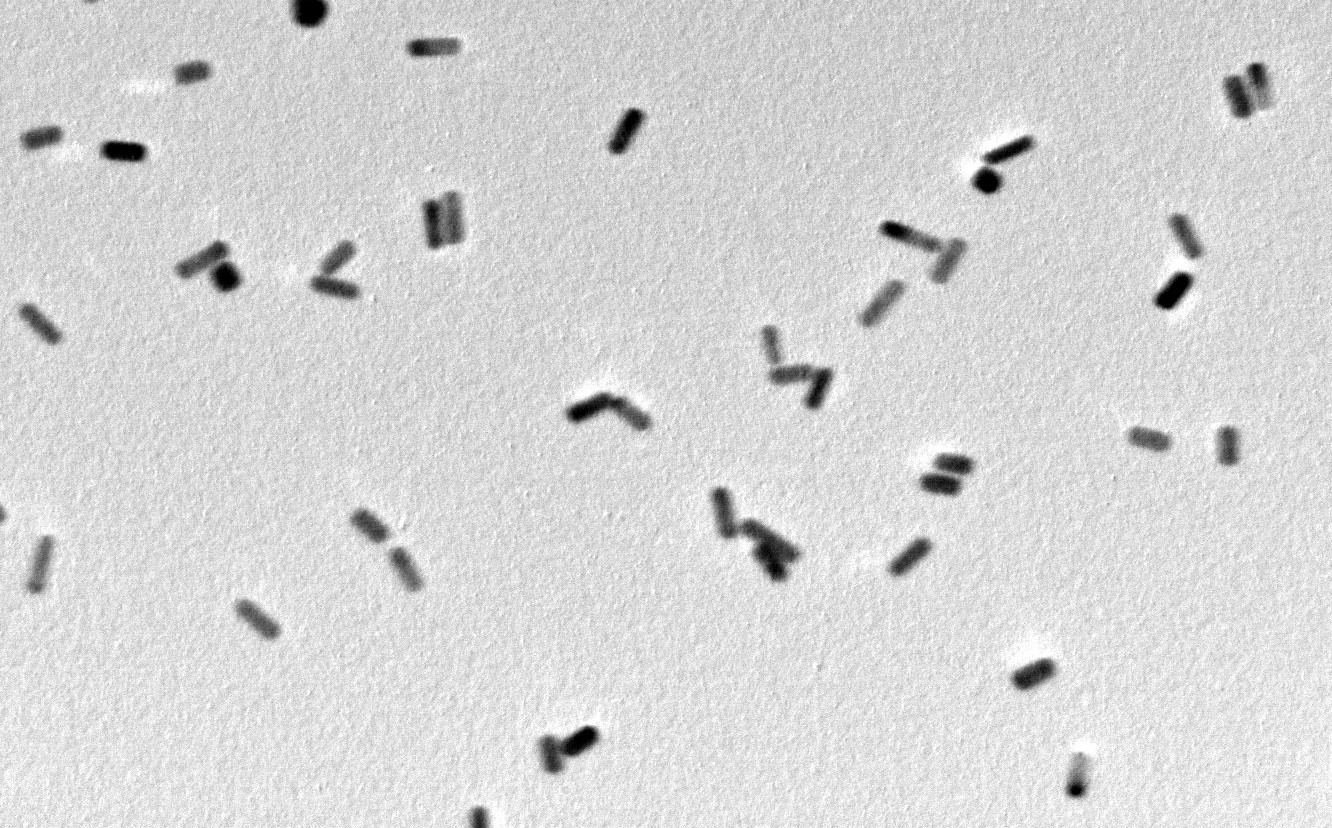
\includegraphics[width=0.5\linewidth]{discNRs.jpg}
    \caption{Bad focused nanorods}~\label{fig:bad_focus}
\end{center}
\end{figure}

In speech about overlapping particles there is also one issue with this which cannot be solved. Some samples contain places with a lot of particles laying on each other. In some extreme cases there is not even possible to see individual particles. This images obviously cannot be used for analysis. Program detects these huge clusters as one particle and it would bring enormous error in results so program have treated these cases removing such huge areas which were detected as one particle. Example of image with this case can be seen on figure \ref{fig:big_spot}.

\begin{figure}[h!]
\begin{center}
    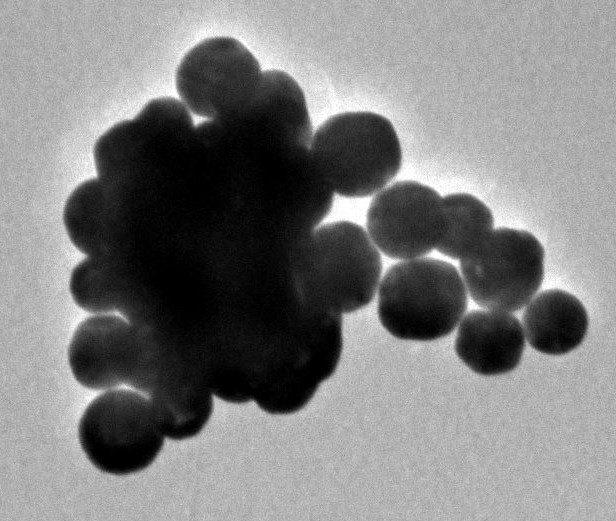
\includegraphics[width=0.5\linewidth]{disc80nm.jpg}
    \caption{Image with huge cluster of particles}~\label{fig:big_spot}
\end{center}
\end{figure}

Last issue which was recorded is fact that microscope computer saves data into jpg format. It is understandable because jpg in compare with tiff has far lesser size, but compresses data and by compressing artifacts may occur. This can be problem in cases where original image have region with zero pixels and compressing causes that pixels with higher value (1, 2, 3 etc.) occur in this region, example of this region is scale bar. In image analysis program scale bar is detected by intensity threshold and artifacts may cause errors in this detection. It was solved by detecting more than just zero pixels and than taking just the biggest reion which is obviously scale bar.

\subsection{Calculations}

The main goals of this project is to create program which can automatically calculate sizes of nanoparticles and shapes of nanorods. Program returns histogram of diameters for nanoparticles and histogram of major and minor axis length for nanorods and also txt file with sizes of all particles, average sizes and for nanorods also aspect ratio. Errors in this section may be cause by all the cases described in chapter \ref{measurment_errors} and \ref{image_errors}. Detecting wrong particles may cause wrong average size, so particles which are too small or too big are removed. Some false particles may still not be removed due to many reasons so it may cause errors in results. Another source of results errors may be in resolution issue. If there is only a few pixels in one particle, accuracy of measurement extremely decreases. On figure \ref{fig:hist2} is example, where number of pixels in one particle was so small, that difference between particles were just in one pixel. This particles have diameter 8 and 9 pixels and when pixels are transformed into size in nanometers, it created this histogram.

\begin{figure}[h!]
\begin{center}
    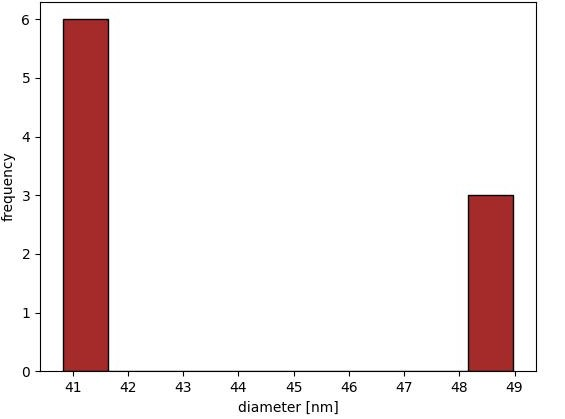
\includegraphics[width=0.8\linewidth]{hist50nm.jpg}
    \caption{Histogram with just two sizes}~\label{fig:hist2}
\end{center}
\end{figure}
        \clearpage
        
        \section{Conclusion}
        \pagestyle{plain}

First goal of the project was to prepare TEM samples which was done using copper grid and potential errors caused by this part of project were evaluated in chapter \ref{measurment_errors} in Discussion. Five samples of nanoparticles of four different sizes were prepared and two samples of nanorods with different peak absorption wavelength were prepared.

Second goal of the project was to get TEM images of nanoparticles and nanorods. Several image of each sample were acquired by TEM by microscope technician. Examples of TEM images are showed in chapter \ref{TEM_images} in Results. Possible measurnemt errors were evaluated in chapter \ref{image_errors_errors} in Discussion.

Third goal of the project was to sugget methods for image segmentatin of these TEM images of nanoparticles and nanorods. Two segmentation methods were chosen on supervisor's recommendation. First method is called watershed transform and it was main method, other method is called hough transform and it was used just for overlapping particles. Both segmentation methods are descibed in chapter \ref{segmentation} in Methods.

Forth goal of the project was to create Python program for automatic analysis of nanoparticles and nanorods from TEM images. Code for this program can be seed in Attachement. Example outputs of program can be seen in chapter \ref{outputs} in Results and were evaluateed in Discussion. Program features were shortly descibed in chapter \ref{program} in Results.

Fifth goal of the project was to create GUI for program.
        \clearpage
    
    %-------------Literatura-------------------
    \clearpage	
    \renewcommand{\refname}{Reference} 	% Přejmenování Reference
    \printbibliography
    \clearpage
    
    %-------------Přílohy----------------------
        
    \end{document}